\documentclass{article}

% if you need to pass options to natbib, use, e.g.:
%     \PassOptionsToPackage{numbers, compress}{natbib}
% before loading neurips_2019

% ready for submission
% \usepackage{neurips_2019}

% to compile a preprint version, e.g., for submission to arXiv, add add the
% [preprint] option:
%     \usepackage[preprint]{neurips_2019}

% to compile a camera-ready version, add the [final] option, e.g.:
\usepackage[nonatbib, final]{neurips_2019}
     

% to avoid loading the natbib package, add option nonatbib:
%     \usepackage[nonatbib]{neurips_2019}

\usepackage[utf8]{inputenc} % allow utf-8 input
\usepackage[T1]{fontenc}    % use 8-bit T1 fonts
\usepackage{hyperref}       % hyperlinks
\usepackage{url}            % simple URL typesetting
\usepackage{booktabs}       % professional-quality tables
\usepackage{amsfonts}       % blackboard math symbols
\usepackage{nicefrac}       % compact symbols for 1/2, etc.
\usepackage{microtype}      % microtypography

\usepackage{float}
\usepackage{graphicx}
\usepackage{subfig}

\usepackage{cite}
\usepackage{booktabs}
\usepackage{tabularx}
\usepackage{graphicx}
\usepackage{caption} 
\usepackage{multirow}
\captionsetup[table]{skip=10pt}

% Default fixed font does not support bold face
\DeclareFixedFont{\ttb}{T1}{txtt}{bx}{n}{12} % for bold
\DeclareFixedFont{\ttm}{T1}{txtt}{m}{n}{12}  % for normal

% Custom colors
\usepackage{color}
\definecolor{deepblue}{rgb}{0,0,0.5}
\definecolor{deepred}{rgb}{0.6,0,0}
\definecolor{deepgreen}{rgb}{0,0.5,0}
\definecolor{light-gray}{gray}{0.95}

\usepackage{listings}
% \usepackage{lmodern}  % for bold teletype font
\usepackage{amsmath}  % for \hookrightarrow
\usepackage{xcolor}   % for \textcolor

% Python style for highlighting
\newcommand\pythonstyle{\lstset{
language=Python,
% basicstyle=\tt,
basicstyle=\ttfamily, columns=fullflexible,
morekeywords={self},              % Add keywords here
keywordstyle=\tt\color{deepblue},
emph={MyClass,__init__,forward,ColumnParallelLinear,RowParallelLinear,ParallelSelfAttention,ParallelCrossEntropy,ParallelTransformerLayer,ParallelTransformer,GPT2, Embedding, ParallelMLP,VocabParallelEmbedding,Linear,Profiler},          % Custom highlighting
emphstyle=\tt\color{deepred},    % Custom highlighting style
stringstyle=\color{deepgreen},
% frame=tb,  
frame=none, % Any extra options here
showstringspaces=false,
breaklines=true,
% ostbreak=\mbox{\textcolor{red}{$\hookrightarrow$}\space},
belowskip=0em,
backgroundcolor = \color{light-gray},
% xleftmargin = .2em,
% framexleftmargin = .2em
}}


% Python environment
\lstnewenvironment{python}[1][]
{
\pythonstyle
\lstset{#1}
}
{}

% Python for external files
\newcommand\pythonexternal[2][]{{
\pythonstyle
\lstinputlisting[#1]{#2}}}

% Python for inline
\newcommand\pyinline[1]{{\pythonstyle\lstinline!#1!}}


\title{Graph Neural Networks For Recommender Systems}

% The \author macro works with any number of authors. There are two commands
% used to separate the names and addresses of multiple authors: \And and \AND.
%
% Using \And between authors leaves it to LaTeX to determine where to break the
% lines. Using \AND forces a line break at that point. So, if LaTeX puts 3 of 4
% authors names on the first line, and the last on the second line, try using
% \AND instead of \And before the third author name.

\author{
  \textbf{Albert Liang}  \\
  Carnegie Mellon University \\
  \texttt{ajliang@cs.cmu.edu} \\
  \And
  \textbf{Tianyu Zhang} \\
  Carnegie Mellon University \\
  \texttt{tianyuz2@andrew.cmu.edu} \\
  \And
  \textbf{Hiroshi Wu} \\
  Carnegie Mellon University \\
  \texttt{bw1@cs.cmu.edu} \\
}

\begin{document}

\maketitle

% \begin{abstract}
% sss
% \end{abstract}


\section{Introduction} \label{intro}

% \textit{TODO: change regression problem to ranking problem}

Recommendation systems are deployed to serve personalized content that is interesting to each individual user on applications such as YouTube, Amazon, and UberEats. Modern recommendation systems leverage deep-learning-based models to better characterize user interests. Designing recommendation models has become an important problem in the machine learning field.

One prominent recommendation problem is the ranking problem: given a set of items for a specific user, we want to rank the items for the user and select a top subset of items in a way that maximizes the relevance of the selected items to the user. This matches the upper-level application logic that, for example, only a small number of videos can be displayed on a user's home feed. More concretely, we have two inputs $u,i$ and an output $r_{ui}$, where $u$ stands for a user, $i$ stands for an item, and $r_{ui}$ is the relevance of the item to the user. We wish to learn a function $f(u,i)$ such that $\hat{r}_{ui}=f(u,i)$ is as close as possible to $r_{ui}$. Given the $r_{ui}$ values for a given $u$ and varying $i$, we are then able to rank them in descending order to obtain items that will most likely interest the given user and recommend those top-ranked items.

Here we will use the MovieLens 100K \cite{movielens} dataset to train and evaluate our models. MovieLens is a series of datasets collected from the MovieLens website where users have rated movies on a rating scale of 1 to 5. These datasets are widely used as benchmark datasets for recommendation systems \cite{DBLP:journals/corr/abs-2011-02260}, making it great forr comparing our models to others. There are different sized MovieLens datasets, and we will use the smallest but most commonly used 100k dataset since it will train faster with limited hardware and have more comparisons available. 

Contextualizing the ranking problem with the MovieLens dataset, $u$ corresponds to users, $i$ corresponds to movies, and $r_{ui}$ corresponds to the rating that user $u$ gave to movie $i$, where $r_{ui}\in\{1,2,3,4,5\}$. However, in this paper, we will discard the concrete value of the rating, and let $r_{ui}=1$ if user $u$ has rated movie $i$ and $0$ otherwise. This modified target is a click-through rate (CTR) type of target, from which the probability of a user interacting with an item, i.e. having watched the movie, can be inferred. We made this choice because CTR could often be a more interesting and useful target to predict in actual industrial applications than regressing on numeric rating \cite{ctr}.


\section{Background}

% \textit{TODO: Briefly summarize the findings from your midway report.}

We implemented five baseline algorithms in the midway report: singular value decomposition (SVD), non-negative matrix factorization (NMF), slope one, k-nearest neighbors (kNN), and random guessing. We benchmarked them on MovieLens with regression metrics RMSE and MAE and obtained results in Table \ref{tab:rmse_results}, \ref{tab:mae_results}. SVD beats the other baselines in both RMSE and MAE. After the midway report, we additionally ran ranking-based metrics on the baseline methods and the results are summarized in Table \ref{tab:baseline-ranking-metrics}. Again, SVD outperforms other baselines except for Recall where kNN wins. Further, we observed that some of these algorithms produced non-trivial improvements to others, and determined there was likely room for improvement even upon SVD.

\begin{table}[H]
    \centering
        \begin{tabular}{|c c c c c|} 
         \hline
         Model & MAP@10 & nDGC@10 & Precision@10 & Recall@10 \\ [0.5ex] 
         \hline\hline
         % LightGCN & 0.034 & 0.153 & 0.145 & 0.093 \\ 
         % \hline
         SVD & \bfseries 0.016 & \bfseries 0.095 & \bfseries 0.087 & 0.037 \\
         \hline
         NMF & 0.002 & 0.024 & 0.025 & 0.010 \\ 
         \hline
         SlopeOne & 0.001 & 0.010 & 0.012 & 0.003 \\ 
         \hline
         kNN & 0.012 & 0.073 & 0.084 & \bfseries 0.049 \\ 
         \hline 
         NormalPredictor & 0.001 & 0.013 & 0.014 & 0.004 \\[1ex] 
         \hline
        \end{tabular}
    \title{sdas}
    \caption{Rank-based evaluation metrics on baselines trained on the \texttt{movielens-100K} dataset. For a detailed definition of these metrics, see section \ref{metrics}}
    \label{tab:baseline-ranking-metrics}
\end{table}

We noted that traditional methods are often limited in expressivity since the models are relatively simple, for example a single matrix. Neural networks by themselves also lack the structure needed to take advantage of the complex structure between user-item ratings and features. We hypothesized that the best of two worlds might be attainable using graph neural networks.

Our dataset is inherently structured as a bipartite graph, with one party the users and the other party the items. Edges between these nodes thus correspond to the ratings user gave to items. Then the message passing and aggregation algorithms applied to this graph is a combination of both the traditional neighborhood method and a neural network. 


\section{Related Work} 

% \textit{Previous work related to your topic that you may have referenced to help guide your project.}

A graph neural network (GNN) is a special class of deep learning models that is design to operate on graph-structured data. Recently, GNNs have been shown to be effective for a wide range of recommendation tasks. A survey on GNNs proposed a taxonomy of the usage of GNN in recommender systems \cite{survey}: \textbf{user-item collaborative filtering} (model the relationships between users and items to make recommendations based on the preferences of similar users), \textbf{sequential recommendation} (model the sequence of items that a user has interacted with in the past to make recommendations based on their previous behavior), \textbf{social recommendation} (model the social relationships between users to make recommendations based on the preferences of friends or other users in a user's social network), and \textbf{knowledge graph-based recommendation} (model the relationships between entities in a knowledge graph to make recommendations based on its structure). We take on the approach to employ GNNs as user-item collaborative filtering models. 

% \begin{itemize}
%     \item \textbf{User-item collaborative filtering}: model the relationships between users and items to make recommendations based on the preferences of similar users.
%     \item \textbf{Sequential recommendation}: model the sequence of items that a user has interacted with in the past to make recommendations based on their previous behavior.
%     \item \textbf{Social recommendation}: model the social relationships between users to make recommendations based on the preferences of friends or other users in a user's social network.
%     \item \textbf{Knowledge graph-based recommendation}: model the relationships between entities in a knowledge graph to make recommendations based on its structure.
% \end{itemize}

We sought inspiration from a variety of GNN architectures. Graph Convolutional Networks (GCN) uses convolutional layers to learn a hierarchical representation of the data, allowing it to effectively capture the complex relationships between nodes in the graph \cite{gcn}. GraphSAGE is a variant of GCN that uses a sample-and-aggregate strategy to learn the node representations \cite{graphsage}, while Graph Attention Networks (GAT) uses self-attention mechanisms to weight the importance of different nodes in the graph \cite{gat}. We studied and broke down the architecture design choices of these GCN variants and apply them as building blocks in the design of our networks. In addition, LightGCN \cite{lightgcn} was originally proposed to simplify the design of Neural Graph Collaborative Filtering (NGCF) \cite{ngcf}. Due to its simple and vanilla architectural design, it suits well as our GNN baseline and building foundation. 

\section{Methods}

% \textit{By the final report, we expect you to have implemented your own ideas beyond the baseline. Additionally, you should describe what work you have completed towards creating a method which beats the
% baseline. In addition to successful approaches, you should briefly detail approaches which you tried and found to not work well. What methods have you completed? What is your motivation behind these techniques (you are encouraged to come up with an original idea of your own or interesting applications rather than simply implementing or applying existing ML algorithms)?}

\subsection{Learning-to-Rank Paradigm}

% \textit{describe embedding, inner product score, rank based on score}

To implement the ranking framework formulated in Section \ref{intro}, we represent a user $u$ through an embedding $e_u=g(u)$, and an item $i$ through an embedding $e_i=g(i)$, where $g$ is an embedding function derived from a GNN. We then take $f=\langle\cdot{,}\cdot\rangle$ to be the inner product of embedding vectors, and thus $$\hat r_{ui} = \langle e_u {,} e_i \rangle$$ 
For a specific user $u$, we obtain $$R_u =\{\hat r_{ui} : \hat r_{ui}=\langle e_u {,} e_i \rangle ~\forall i \}$$
We then produce a ranking of all items for user $u$ by $$\text{Ranking}(u, I) = I[\text{argsort}(R_u)]$$ where $I$ is the list of all items.


\subsection{Graph Node Embedding}

The key to the above ranking paradigm is the embedding function $g$ that we will implement using GNN. A graph embedding architecture typically consists of these four main mechanisms:

\begin{itemize}
    \item \textbf{Graph Construction}. This step constructs a graph from the data so that we can actually train our graph neural network. In the case of user-item collaborative filtering, the simplest paradigm is to construct a bipartite graph, with users belonging to one half and items belonging to the other, with edges signifying interactions. In sequential recommendation, one might use a directed graph to represent causal and temporal relations. In knowledge graph based recommendation, graphs may be augmented with information, and different types of nodes and edges may represent different types of knowledge present in the graph.
    \item \textbf{Neighborhood Aggregation}. This step learns how to aggregate information from neighbor nodes. For example, one could compute the weighted sum of the embeddings of the neighbors of a given node, where the weights are learned by the GNN. The output from this step can be thought of as the aggregated representation of the neighbors.
    \item \textbf{Information Update}. This step learns how to combine the aggregated representation of the neighbor embeddings with the current embeddings in order to create the next embedding for a given node. For example, one may use a simple element-wise addition to combine the output from the neighborhood aggregation step with the current embeddings.
    \item \textbf{Final Node Representation}. This step combines all previous embeddings (i.e. every layer) into a single, final embedding for each node. For example, one could concatenate together the embeddings from every layer. Once the final node representation is computed, it is used as input to a prediction model.
\end{itemize}

\begin{figure}[H]
    \centering
    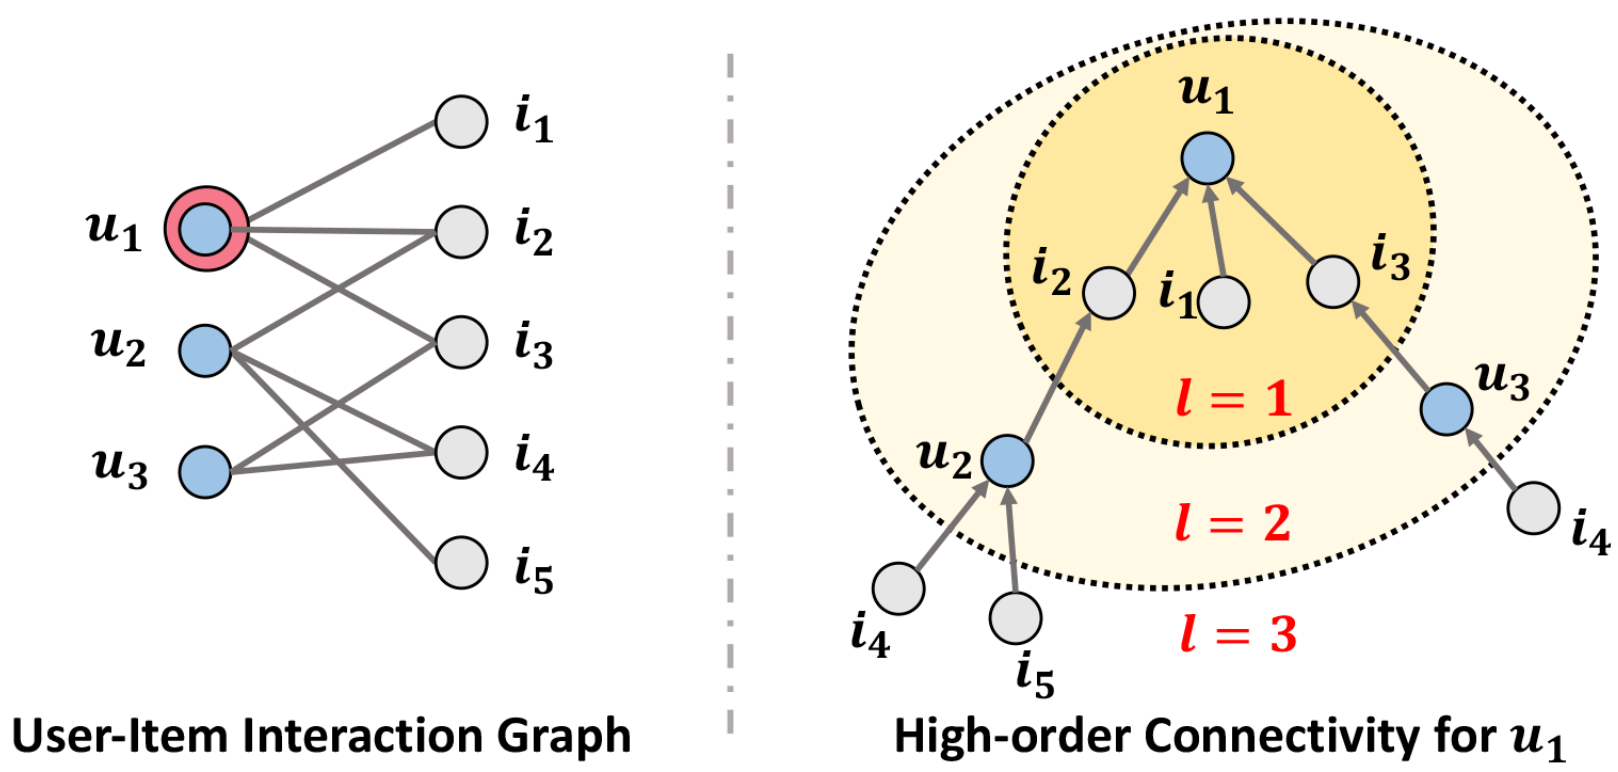
\includegraphics[width=.6\textwidth]{figs/ngcf-architecture.png}
    \caption{An illustration of the user-item interaction graph and the high-order connectivity by \cite{ngcf}. The figure visualizes how the embeddings for user $u_1$ are propagated through the graph.}
    \label{fig:user-item-interact-graph}
\end{figure}

In the following sub-sections, we separately explore different algorithms for each of the above mechanisms. Each combination of a Neighborhood Aggregation algorithm, an Information Update algorithm, and a Final Node Representation algorithm would yield a different GNN. 

\subsubsection{Graph Construction}

The graph construction to choose from depends heavily on what information is given in the dataset. In Movielens 100k, this consists almost entirely of users' ratings on movies, with minimal data on attributes of each user or each movie. Since the useful information consists only of raw user-item interactions, we are only able to do user-item collaborative filtering. Hence, we will start with a bipartite user-item interaction graph.

Wu, et. al., \cite{survey} notes that we can add edges or nodes to this graph to increase the connectivity between certain nodes. Multi-GCCF \cite{multigccf} adds edges between two-hop neighbors to facilitate information passing among related users. However since our architecture is based on LightGCN which passes unaltered information very well along paths, it is not theoretically necessary to further increase connectivity. DGCF \cite{dgcf} adds nodes to express intent and then further processes the graph. We will adapt this idea to address one of our weaknesses with our proposed model, which is that it does not take into consideration any user or item features. We add feature nodes to the graph and for each feature node add edges to all users or items whose features are sufficiently close. This may be done using any clustering algorithm, such as k-means. Here since we do not have much features, we directly featurize the items based on its reported genre. Each movie genre is given a node, and movies within the same genre are connected to it. The intention is that this allows users nodes to receive information from movies of similar genres to the ones the user rated, which users might prefer.

\subsubsection{Neighborhood Aggregation}
\label{neighborhood_aggregation}

We adopted two mechanisms to aggregate node information to compute embedding of a given layer. 
\begin{itemize}
    \item \textbf{Weighted Sum}, which is a simple weighted sum aggregator defined as: $$n_u^{(l+1)}=\sum_{i\in \mathcal{N}_u} \frac{1}{\sqrt{|\mathcal{N}_u|} \sqrt{|\mathcal{N}_i|}} h_i^{(l)} \text{ for } l \in 0, 1, \hdots, K - 1$$
    where $\frac{1}{\sqrt{|\mathcal{N}_u|} \sqrt{|\mathcal{N}_i|}}$ is the normalizing factor that adjusts the scale of embeddings based on graph connectivity, which is known as the renormalization trick proposed by GCN \cite{gcn}.

    Notice that in this setting, the neighborhood aggregation function is just a linear transformation of the previous layer. Therefore, we can derive a closed form solution of the aggregated representation in terms of the previous layer in matrix notation, which is significantly faster to compute compared to the naive implementation of the weighted sum as a for loop. Specifically, let $R \in \mathbb{R}^{m \times n}$ denote the interaction matrix where $R_{ui}$ is 1 if user $u$ has a rating for movie $i$ and 0 otherwise. Here $m$ and $n$ are the number of users and movies respectively. Then, the adjacency matrix of the bipartite user-movie interaction graph can be written as
    \begin{align*}
        A =
        \begin{pmatrix}
        \mathbf{0} & R \\
        R^\top & \mathbf{0}
        \end{pmatrix}
    \end{align*}
    Treating this as a classical matrix factorization problem, we arrive at the closed form solution of the aggregation representation:
    \begin{align*}
        N^{(l+1)} = \left( D^{-\frac{1}{2}} A D^{-\frac{1}{2}} \right) H^{(l)} \text{ for } l \in 0, 1, \hdot, K - 1
    \end{align*}
    where $D \in \mathbb{R}^{(m+n) \times (m+n)}$ is a diagonal matrix such that the $i$th diagonal entry denotes the number of non-zero entries in the $i$th row of $A$.
    
    \item \textbf{Attention}, which uses the attention mechanism to compute weights for each node. Specifically, we add a graph attention layer that borrows its design from GAT \cite{gat}. 
    
    The graph attention layer is parametrized by a weight matrix $W \in \mathbb{R}^{F' \times F}$ where $F, F'$ are input and output feature dimensions, respectively, and a shared set of attention weights that perform self-attention on the nodes $a \in \mathbb{R}^{2F'}$. 

    Concretely, the attention weights between node $u$ and $i$ is $$\alpha_{ui} = \text{softmax} (e_{ui}) = \frac{\text{exp}(\text{LeakyReLU} (a^T [Wh_u \oplus Wh_i]) )}{\sum_{j\in \mathcal{N}_u}  \text{exp}(\text{LeakyReLU} (a^T [Wh_u \oplus Wh_j]) )}$$
    where $\oplus$ is the concatenation operator. Note that the above equation incorporates graph connectivity information by performing masked attention, i.e. we only compute $e_{ui}$ for nodes $i\in \mathcal{N}_u$. We temporarily dropped the ${(l)}$ superscript for notational simplicity as everything in scope here occurs on the same layer.

    Now with the attention weights, we compute the final embedding as follows: $$n_u^{(l + 1)} = \sigma ( \sum_{i\in \mathcal{N}_u} \alpha_{ui} W h_i^{(l)}  ) \text{ for } l \in 0, 1, \hdots, K - 1 $$ where we chose the nonlineariy $\sigma$ to be the Exponential Linear Function (ELU).
\end{itemize}

\subsubsection{Information Update}

For the Information Update module, we implemented three different algorithms:
\begin{itemize}
    \item \textbf{Multiple Linear}, which computes the next embedding for a given node as a push-forward of the aggregated neighbor embeddings through a linear layer activated by LeakyRelu. Mathematically, this is defined as:
    $$
    h_u^{(l+1)} = \mbox{LeakyRelu}(n_u^{(l)} W^{(l)} + b^{(l)}) \text{ for } l \in 0, 1, ..., K
    $$
    where $n_u^{(l)}$ and $h_u^{(l+1)}$ are the aggregated neighbor embeddings and the next embedding for node $u$ at layer $l$, respectively. $W^{(l)}$ and $b^{(l)}$ are the weight and bias parameters for the linear layer at layer $l$, respectively.
    \item \textbf{Single Linear}, which is the same as \textit{Multiple Linear} except that the same LeakyRelu activated linear layer is shared among all layers. Mathematically, this is defined as:
    $$
    h_u^{(l+1)} = \mbox{LeakyRelu}(n_u^{(l)} W + b) \text{ for } l \in 0, 1, ..., K - 1
    $$
    Notice that the same $W$ and $b$ are used for all layers.
    \item \textbf{Identity}, which simply sets the next embedding for a given node to be its aggregated neighbor embeddings. Mathematically, this is defined as:
    $$
    h_u^{(l+1)} = n_u^{(l)} \text{ for } l \in 0, 1, ..., K - 1
    $$
\end{itemize}

\subsubsection{Final Node Representation} \label{final_node_representation}

Four different choices of final node representation were chosen to be compared. Let $h_u^*$ be the final representation, then we can choose function $f$ such that $h_u^*=f(h_u^{(0)},h_u^{(1)},\hdots,h_u^{(K)})$.

\begin{itemize}
    \item \textbf{Concatenation}, which simply concatenates embeddings from all layers into a single embedding.
    $$h_u^*=h_u^{(0)} \oplus h_u^{(1)} \oplus \cdots \oplus h_u^{(K)}$$
    This means that the number of dimensions of the embedding is multiplied by the number of layers $+1$, which can be very big. This is the approach used by NGCF \cite{ngcf}.
    \item \textbf{Mean}, which averages the embeddings from each layer instead of concatenating them. Mathematically, this is
    $$h_u^*=\frac{1}{K+1}\sum_{l=0}^Kh_u^{(l)}$$
    This avoids the explosion in embedding dimensions, but risks losing some information in the process, as it is unclear whether such a simple combination of embeddings from different layers can produce a more meaningful embedding. This is the approach used by LightGCN \cite{lightgcn}.
    \item \textbf{Weighted Sum}, which is a weighted sum of the embeddings from each layer.
    $$h_u^*=\sum_{l=0}^K\alpha^{(l)}h_u^{(l)}$$
    where each $\alpha$ is a learnable parameter. This approach is mentioned in LightGCN \cite{lightgcn} but is not fully explored.
    
    In practice we do not want the norm of the embeddings to explode, so we keep it as a \textit{convex} weighted sum by using a softmax over the alphas.
    $$h_u^*=\frac{\sum_{l=0}^K (\exp(\alpha^{(l)})h_u^{(l)})}{\sum_{l=0}^K \exp(\alpha^{(l)})}$$
    \item \textbf{Self-Attention}, which is a convex weighted sum of embeddings from each layer, except that the weights are computed through a self-attention mechanism. This attention is inspired by the mechanism used in the transformers architecture \cite{transformer}, and is different from graph attention used in neighborhood aggregation (Section \ref{neighborhood_aggregation}). Transformers define attention to be
    $$\text{Attention}(Q,K,V)=\text{softmax}(\frac{QK^T}{\sqrt{d_k}})V$$
    where $Q$ is a query vector, $K$ is a key vector, $V$ is a value vector, and $d_k$ is the dimensions of the $K$. The result is a convex combination of the value vectors, with weights determined by interactions between query and key vectors. Self-attention simply sets $Q=K=V$ to the embedding in question. We then employ a few modifications to this scheme to fit our use case.
    \begin{enumerate}
        \item This mechanism traditionally computes attention results for all $K+1$ embeddings to produce $K+1$ results. We only need one final result, so we choose to only use the first result and discard the rest.
        \item We employ a trainable linear feature transformation for the query vector only, so attention can learn what to attend to.
        \item We discard the $1/\sqrt{d_k}$ factor since softmax already normalizes the results.
    \end{enumerate}
    Combining these, we obtain
    $$h_u^*=\frac{\sum_{l=0}^K (\exp(\langle h_u^{(0)}W_A, h_u^{(l)}\rangle)h_u^{(l)})}{\sum_{l=0}^K \exp(\langle h_u^{(0)}W_A, h_u^{(l)}\rangle)}$$
    where $W_A$ is a trainable feature transformation.
\end{itemize}

\subsection{Ranking Score Prediction}

With the final learned embeddings output from the final node representation (defined in Section \ref{final_node_representation}) for users and movies, we extract them from the embedding layer of the GNN and compute the scores for recommending movie $i$ to user $u$ as simply their inner product: $\hat r_{ui} = \langle e_u {,} e_i \rangle$.
These ranking scores would be used to compute the loss function (as defined in \ref{bpr_loss}), which allows us to optimize the GNN weights via back propagation.

\subsection{Loss Function and Training} \label{bpr_loss}

We use the Bayesian Personalized Ranking (BPR) loss, a loss designed to train on implicit feedback such as clicks \cite{bprloss}, to train our GNNs. The formula for BPR loss is given as follows:
\begin{align*}
    L_{\mbox{BPR}} = - \sum_{u = 1}^M \sum_{i \in \mathcal{N}_u} \sum_{j \notin \mathcal{N}_u} \ln \sigma(\hat{r}_{ui} - \hat{r}_{uj}) + \lambda \| \mathbf{E}^{(0)} \|^2
\end{align*}
where $\lambda$ is a tuning parameter for the $L_2$ regularization on the initial embedding weights. Intuitively, BPR is a pairwise loss that encourages the prediction of an observed entry to be higher than its unobserved counterparts. We optimize this loss using the Adam \cite{adam} optimizer.

% \subsection{GNN 1: LightGCN}

% The LightGCN model was originally proposed in \cite{lightgcn} to simplify the design of Neural Graph Collaborative Filtering (NGCF), which was proposed earlier in \cite{ngcf}. Specifically, it includes only the most essential components in NGCF -- neighborhood aggregation -- for collaborative filtering. Due to its simplicity, we decided to implement it as our first GNN and adapt it to the MovieLens dataset.

% \subsubsection{LightGCN: Model Definition}

% LightGCN learns the embeddings for the users and movies by iteratively applying graph convolution on the user-item interaction graph, as depicted in Figure \ref{fig:user-item-interact-graph}. Note that the user-item interaction graph is assume to be bipartite, so the user embeddings are updated only using the movies embeddings and vice versa.

% Figure \ref{fig:light-gcn-architecture} summarizes the overall model architecture of LightGCN. In the sections below, we describe each component of this architecture in detail and also present a mathematical overview of the model training procedure.

% \textbf{Light Graph Convolution (LGC)}

% In contrast to NGCF, the graph convolution operation in LightGCN is just a simple weighted sum aggregator, abandoning the use of feature transformation and nonlinear activation. Mathematically, the graph convolution operation is defined as:
% \begin{align*}
%     \mathbf{e}_u^{(k+1)} = \sum_{i \in \mathcal{N}_u} \frac{\mathbf{e}_i^{(k)}}{\sqrt{| \mathcal{N}_u | | \mathcal{N}_i | }} \\
%     \mathbf{e}_i^{(k+1)} = \sum_{u \in \mathcal{N}_i} \frac{\mathbf{e}_u^{(k)}}{\sqrt{| \mathcal{N}_i | | \mathcal{N}_u | }}
% \end{align*}
% where the normalization term $\frac{1}{\sqrt{|\mathcal{N}_i| |\mathcal{N}_u|}}$ helps avoid increasing the scale of the embeddings with more graph convolution operations. \cite{lightgcn}

% \textbf{Layer Combination (Weighted Sum)}

% After $K$ layers of graph convolutions, the final user/movie embedding is obtained as a weighted average of the embeddings from layers $0$ through $K$:
% \begin{align*}
%     \mathbf{e}_u = \sum_{k = 0}^K \alpha_k \mathbf{e}_u^{(k)} \\
%     \mathbf{e}_i = \sum_{k = 0}^K \alpha_k \mathbf{e}_i^{(k)}
% \end{align*}
% where $\alpha_k \geq 0$ is the weight assigned to the embedding from each layer. In \cite{lightgcn}, the authors found that setting $\alpha_k \sim \mbox{Uniform}(0, \frac{1}{K + 1})$ achieves good performance, so we will set $\alpha_k \sim \mbox{Uniform}(0, \frac{1}{K+1})$ in our implementation as well.

% \textbf{Ranking Score Prediction}

% With the final learned embeddings for the users and the movies, LightGCN predicts the ranking score \cite{lightgcn} for recommending movie $i$ to user $u$ as simply their inner product:
% \begin{align*}
%     \hat{y}_{ui} = \mathbf{e}_u^\top \mathbf{e}_i
% \end{align*}

% \textbf{Loss Function}

% In \cite{lightgcn}, the authors train LightGCN using the Bayesian Personalized Ranking (BPR) loss:
% \begin{align*}
%     L_{\mbox{BPR}} = - \sum_{u = 1}^M \sum_{i \in \mathcal{N}_u} \sum_{j \notin \mathcal{N}_u} \ln \sigma(\hat{y}_{ui} - \hat{y}_{uj}) + \lambda \| \mathbf{E}^{(0)} \|^2
% \end{align*}
% where $\lambda$ is a tuning parameter for the $L_2$ regularization. Intuitively, BPR is a pairwise loss that encourages the prediction of an observed entry to be higher than its unobserved counterparts. In our implementation, we employ the BPR loss function in conjunction with the Adam \cite{adam} optimizer.

% \textbf{Mathematical Overview of the Training Procedure} \cite{lightgcn}

% Notice that the only learnable parameter in LightGCN is the initial user/movie embeddings $\mathbf{E}^{(0)} \in \mathbb{R}^{(M + N) \times T}$. Here, $M$, $N$, and $T$ denotes the number of users, the number of movies, and the embedding size respectively. Since each graph convolution is just a linear transformation of the previous layer, we can derive a closed form solution of the final embeddings $\mathbf{E}$ in terms of the initial embeddings $\mathbf{E}^{(0)}$.

% Let $\mathbf{R} \in \mathbb{R}^{M \times N}$ denote the interaction matrix where $\mathbf{R}_{ui}$ is 1 if user $u$ has a rating for movie $i$ and 0 otherwise. Then, we know the adjacency matrix of the bipartite user-movie interaction graph is
% \begin{align*}
%     \mathbf{A} =
%     \begin{pmatrix}
%     \mathbf{0} & \mathbf{R} \\
%     \mathbf{R}^\top & \mathbf{0}
%     \end{pmatrix}
% \end{align*}

% Treating this as a classical matrix factorization problem, we arrive at the propagation rule:
% \begin{align*}
%     \mathbf{E}^{(k+1)} = \left( \mathbf{D}^{-\frac{1}{2}} \mathbf{A} \mathbf{D}^{-\frac{1}{2}} \right) \mathbf{E}^{(k)}
% \end{align*}
% where $\mathbf{D} \in \mathbb{R}^{(M + N) \times (M + N)}$ is a diagonal matrix such that the $i$th diagonal entry denotes the number of non-zero entries in the $i$th row of $\mathbf{A}$. Denote $\mathbf{\tilde{A}} := \mathbf{D}^{-\frac{1}{2}} \mathbf{A} \mathbf{D}^{-\frac{1}{2}}$, we conclude that
% \begin{align*}
% \mathbf{E} &= \alpha_0 \mathbf{E}^{(0)} + \alpha_1 \mathbf{E}^{(1)} + \alpha_2 \mathbf{E}^{(2)} + \hdots + \alpha_K \mathbf{E}^{(K)} \\
% &= \alpha_0 \mathbf{E}^{(0)} + \alpha_1 \mathbf{\tilde{A}} \mathbf{E}^{(0)} + \alpha_2 \mathbf{\tilde{A}}^2 \mathbf{E}^{(0)} + \hdots + \alpha_K \mathbf{\tilde{A}}^K \mathbf{E}^{(0)}
% \end{align*}
% is the closed form solution of the final embeddings $\mathbf{E}$, which we can then feed into the BPR loss function by generating the ranking score predictions.`

\section{Results} \label{results}

\textit{Your experimental results. Show plots of the performance of your algorithms and interpret what they mean. Be sure to label and explain this clearly. Describe how the current results in each of the experiments align with your expectations. What metrics did you use for evaluation? How do your results compare to prior work?}

\subsection{Rank-based Metrics for Model Evaluation} \label{metrics}

% \textit{TODO: cut content, we don't need one page to describe these metrics; can probably move detailed descriptions into appendix and only retain math formulas.} % TZ: I moved metrics math to the appendix.

To evaluate our GNNs and benchmark it against the baselines, we will compare their performance in predicting the relative ranking of the top K items for a user. This is known as the Learning-to-Rank problem \cite{learning_to_rank}. As with most other problems, there is not a single metric that is the absolute best. We evaluate our models with four different rank-based metrics, namely Precision @ K, Recall @ K, Mean Average Precision (MAP) @ K, and Normalized Discounted Cumulative Gain (nDCG) @ K. Their exact mathematical defintiion can be found in Appendix \ref{rank-metrics-def}. Throughout this report, we set $K = 10$, which is a reasonable value for the movie recommendation setting.

Note that different metrics may be better suited for different applications. For instance, MAP is a good metric when the order of the returned recommendation batch is not important whereas nDCG is preferable when we do care about the order. In fact, even for different recommendation stages inside a single application, different metrics may be better suited. Recall may be important for the initial retrieval stage while precision is more important for the final ranking stage. It's often helpful to examine multiple metrics together to understand the performance of a ranking algorithm holistically. Nevertheless, we place a higher emphasis on nDCG which is arguably the more well-rounded end-to-end ranking metric out of the four.

\subsection{Rank-based Metrics for Top Performing Architectures}

\begin{figure}[H]
    \centering
    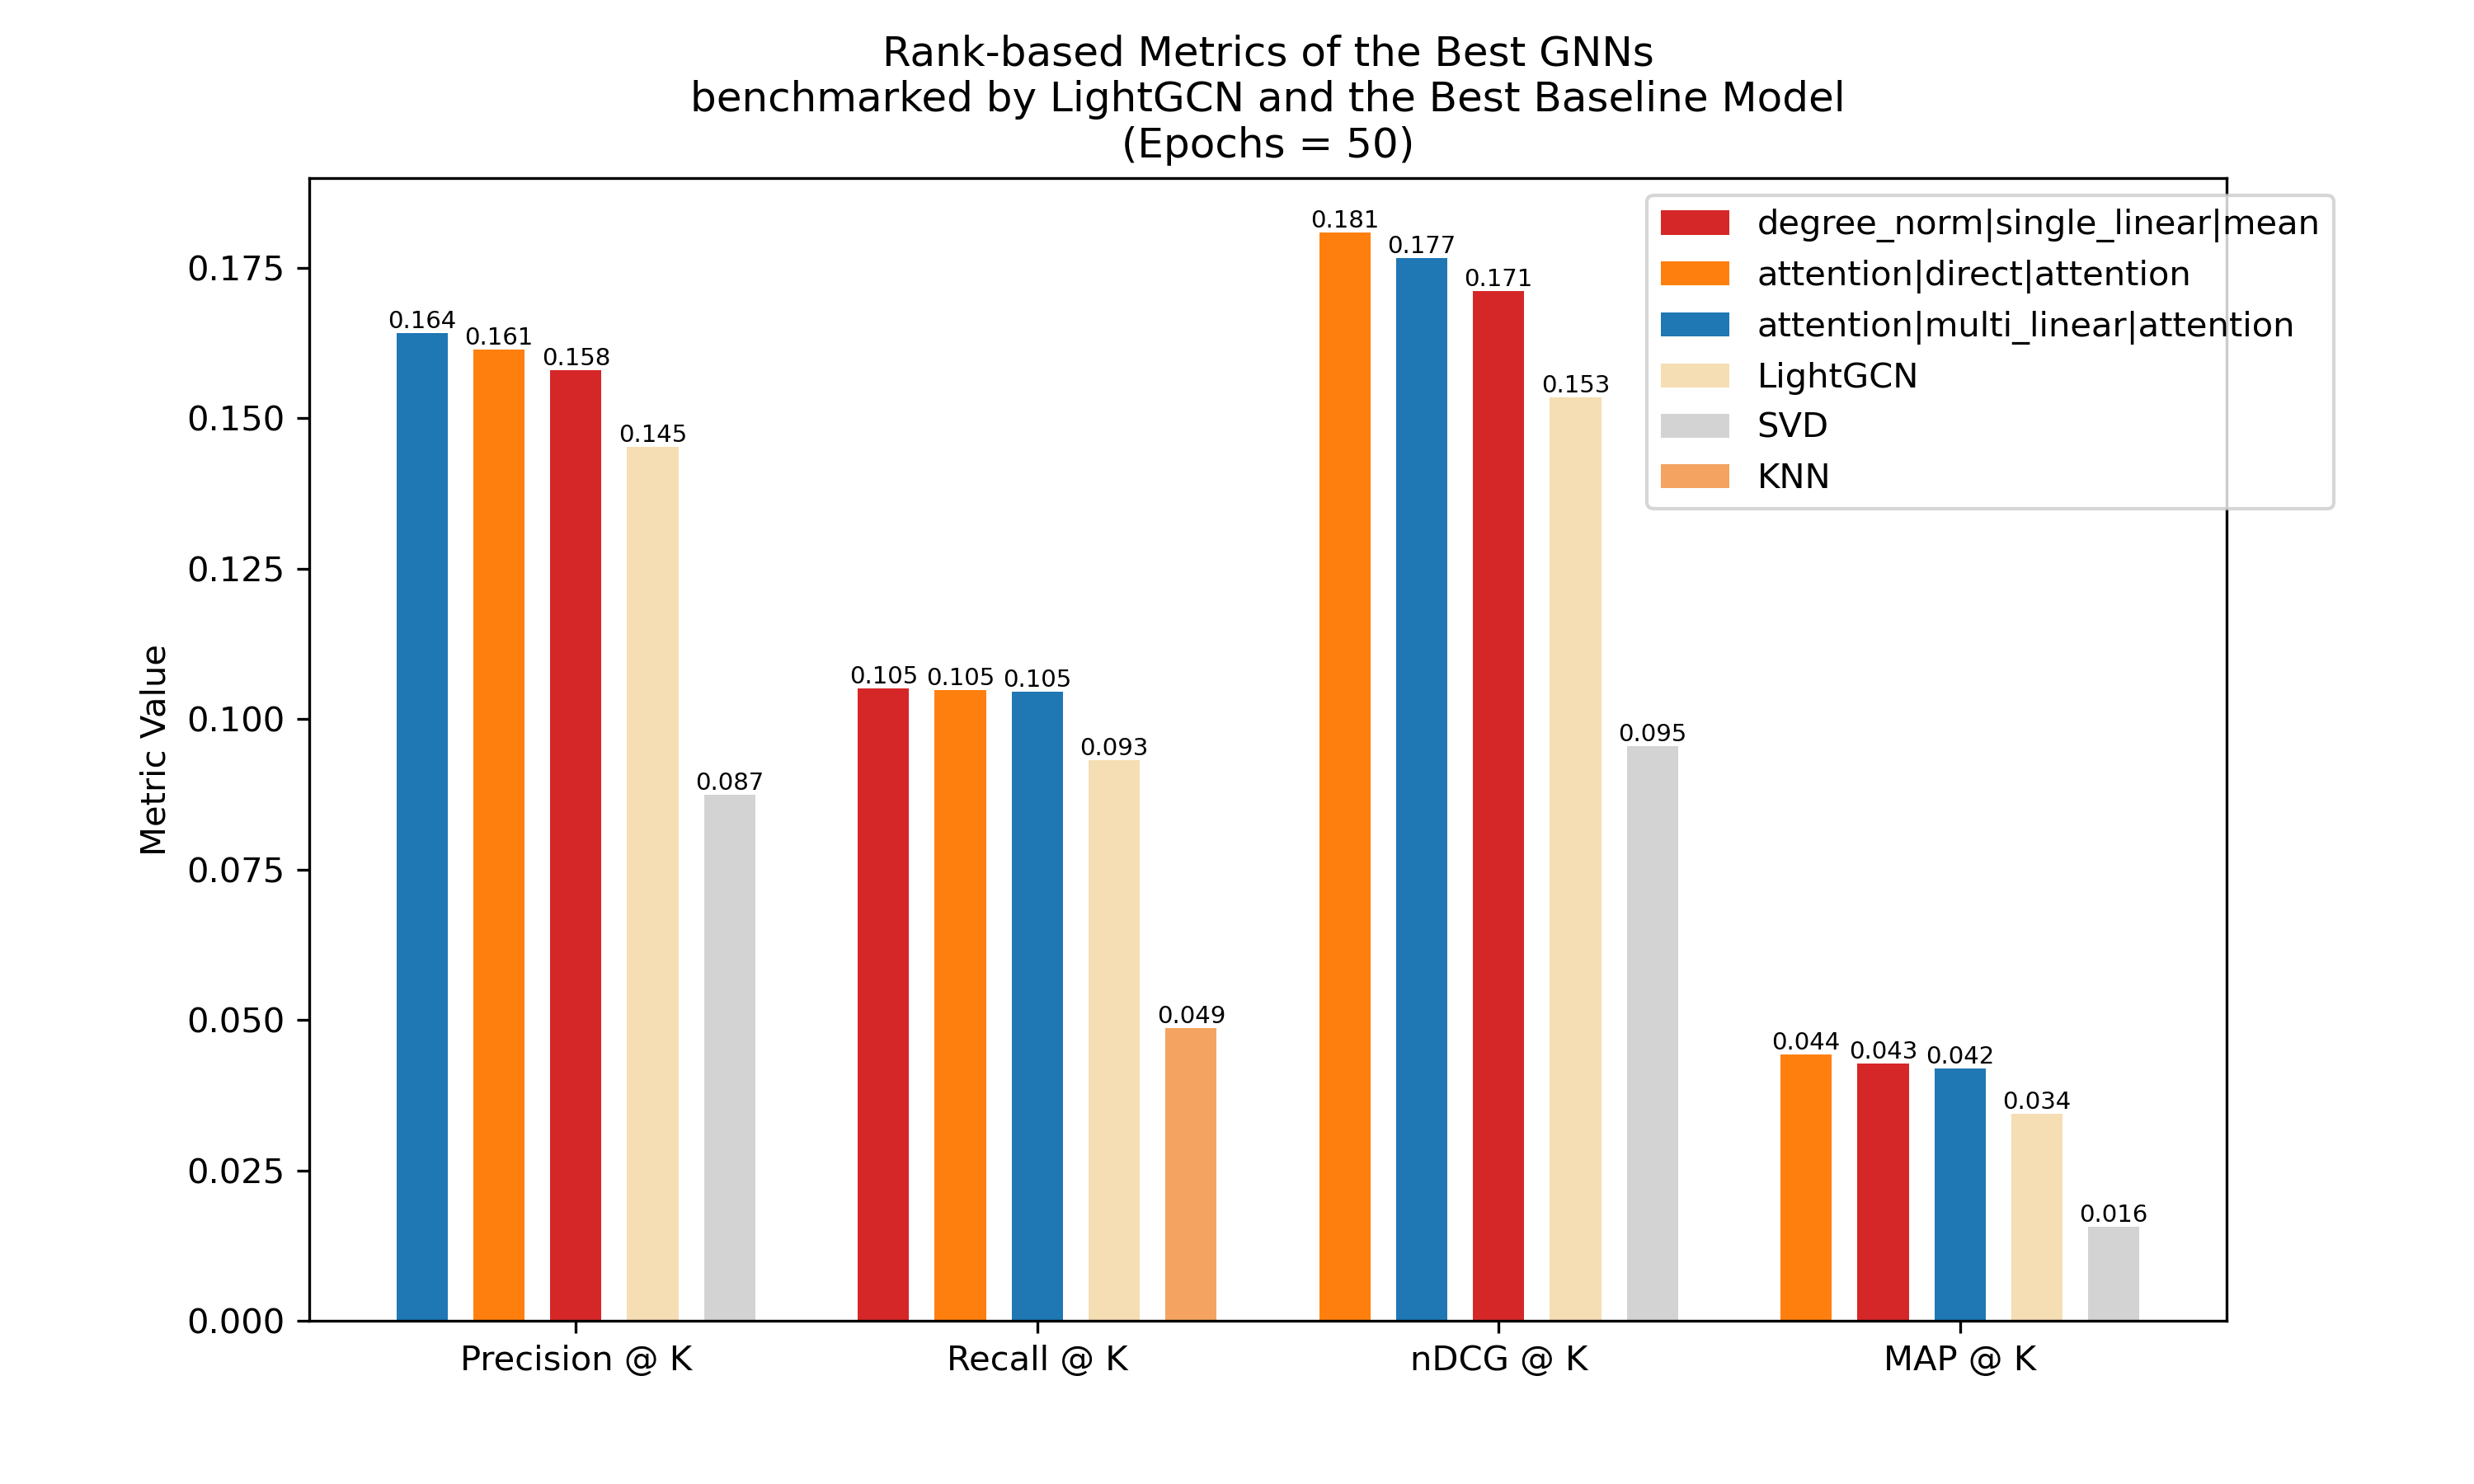
\includegraphics[width=.8\textwidth]{figs/best_models_and_baselines.png}
    \caption{}
    \label{fig:metrics-overall}
\end{figure}


\subsection{Rank-based Metrics for Individual Mechanisms}

\subsubsection{With Vanilla Other Mechanisms}

\begin{figure}[H]
    \centering
    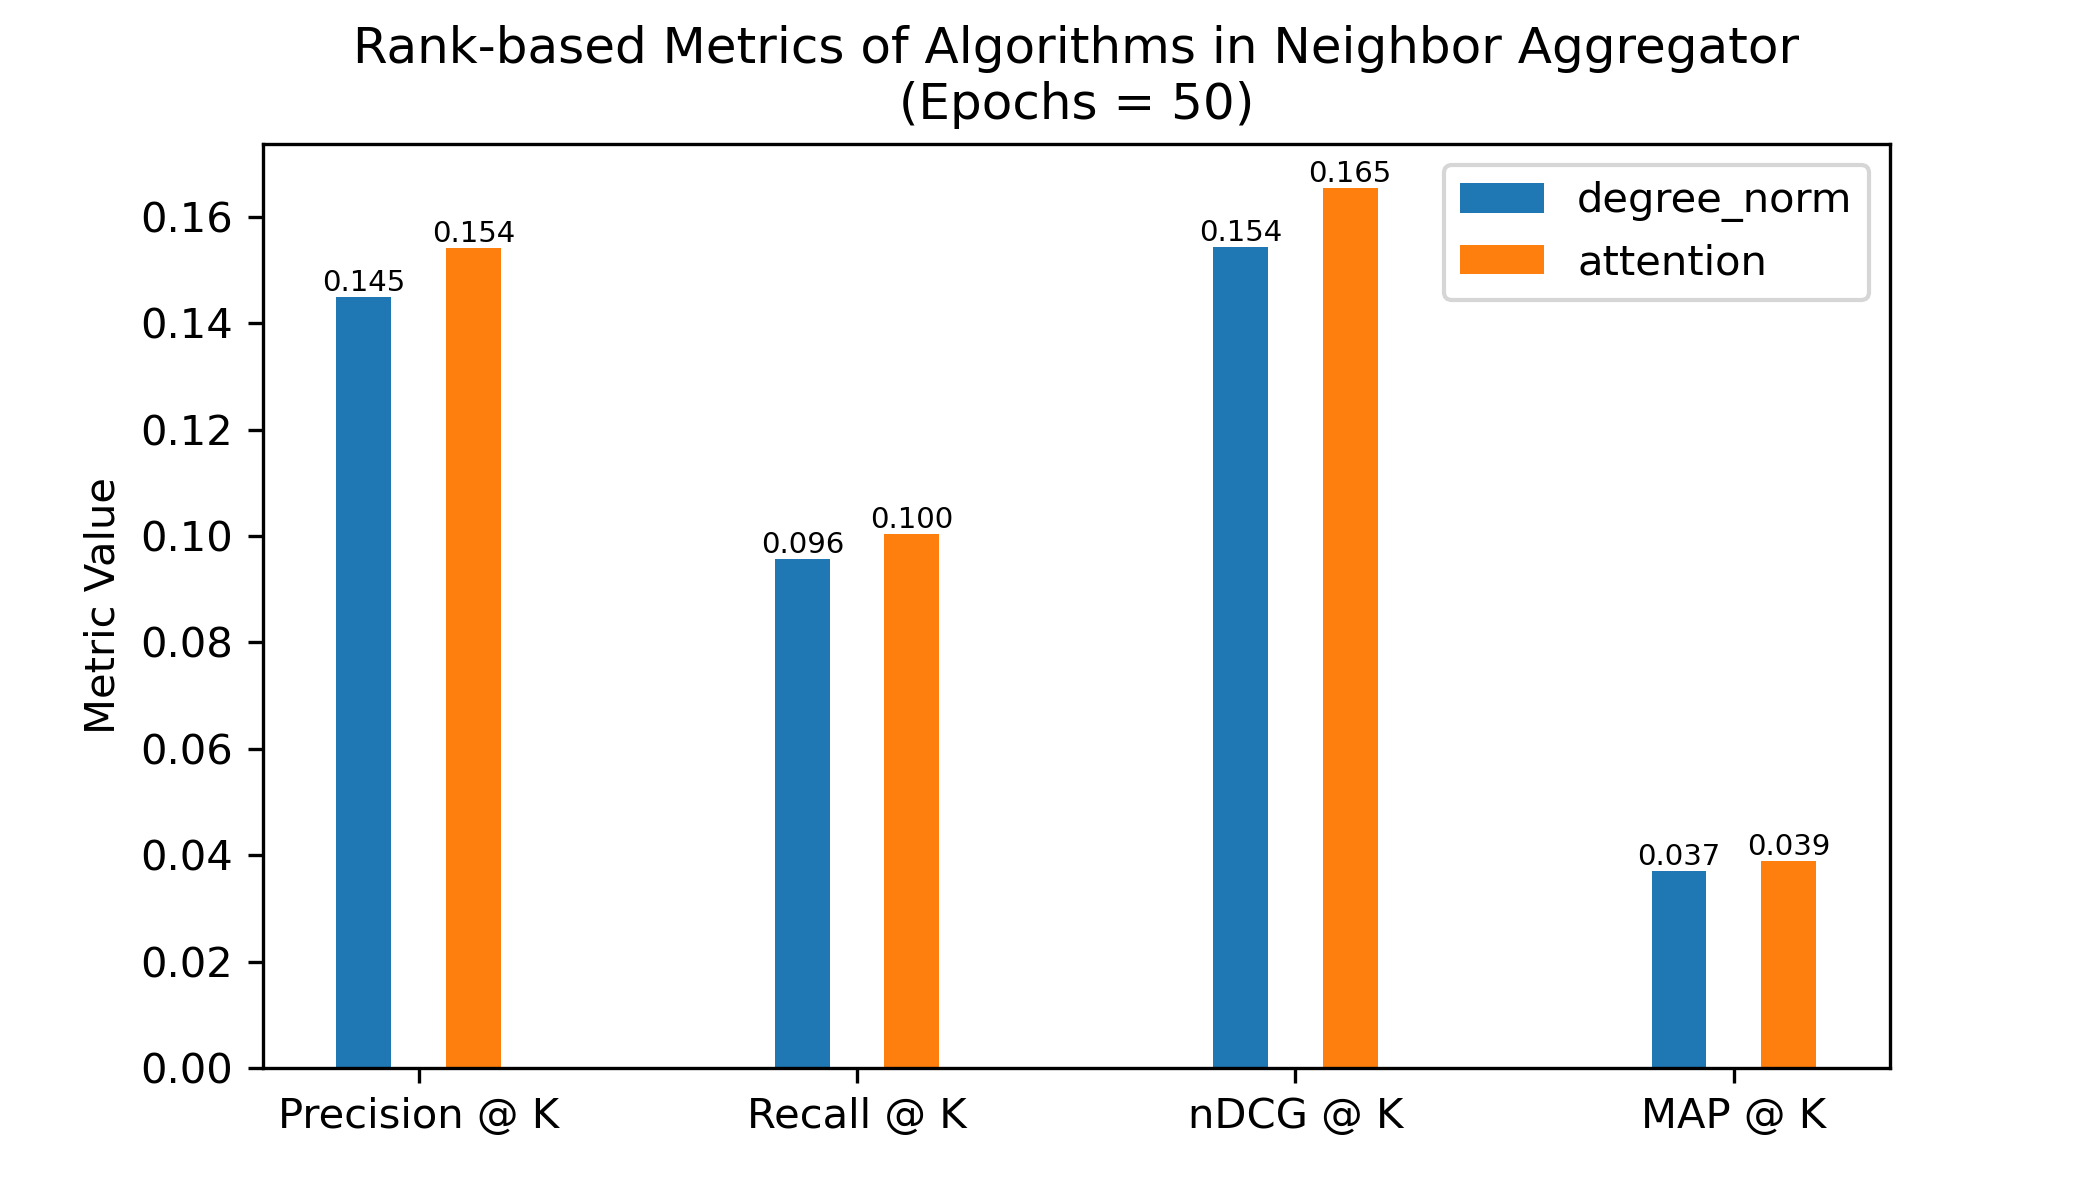
\includegraphics[width=.48\textwidth]{figs/neighbor_aggregator.png}
    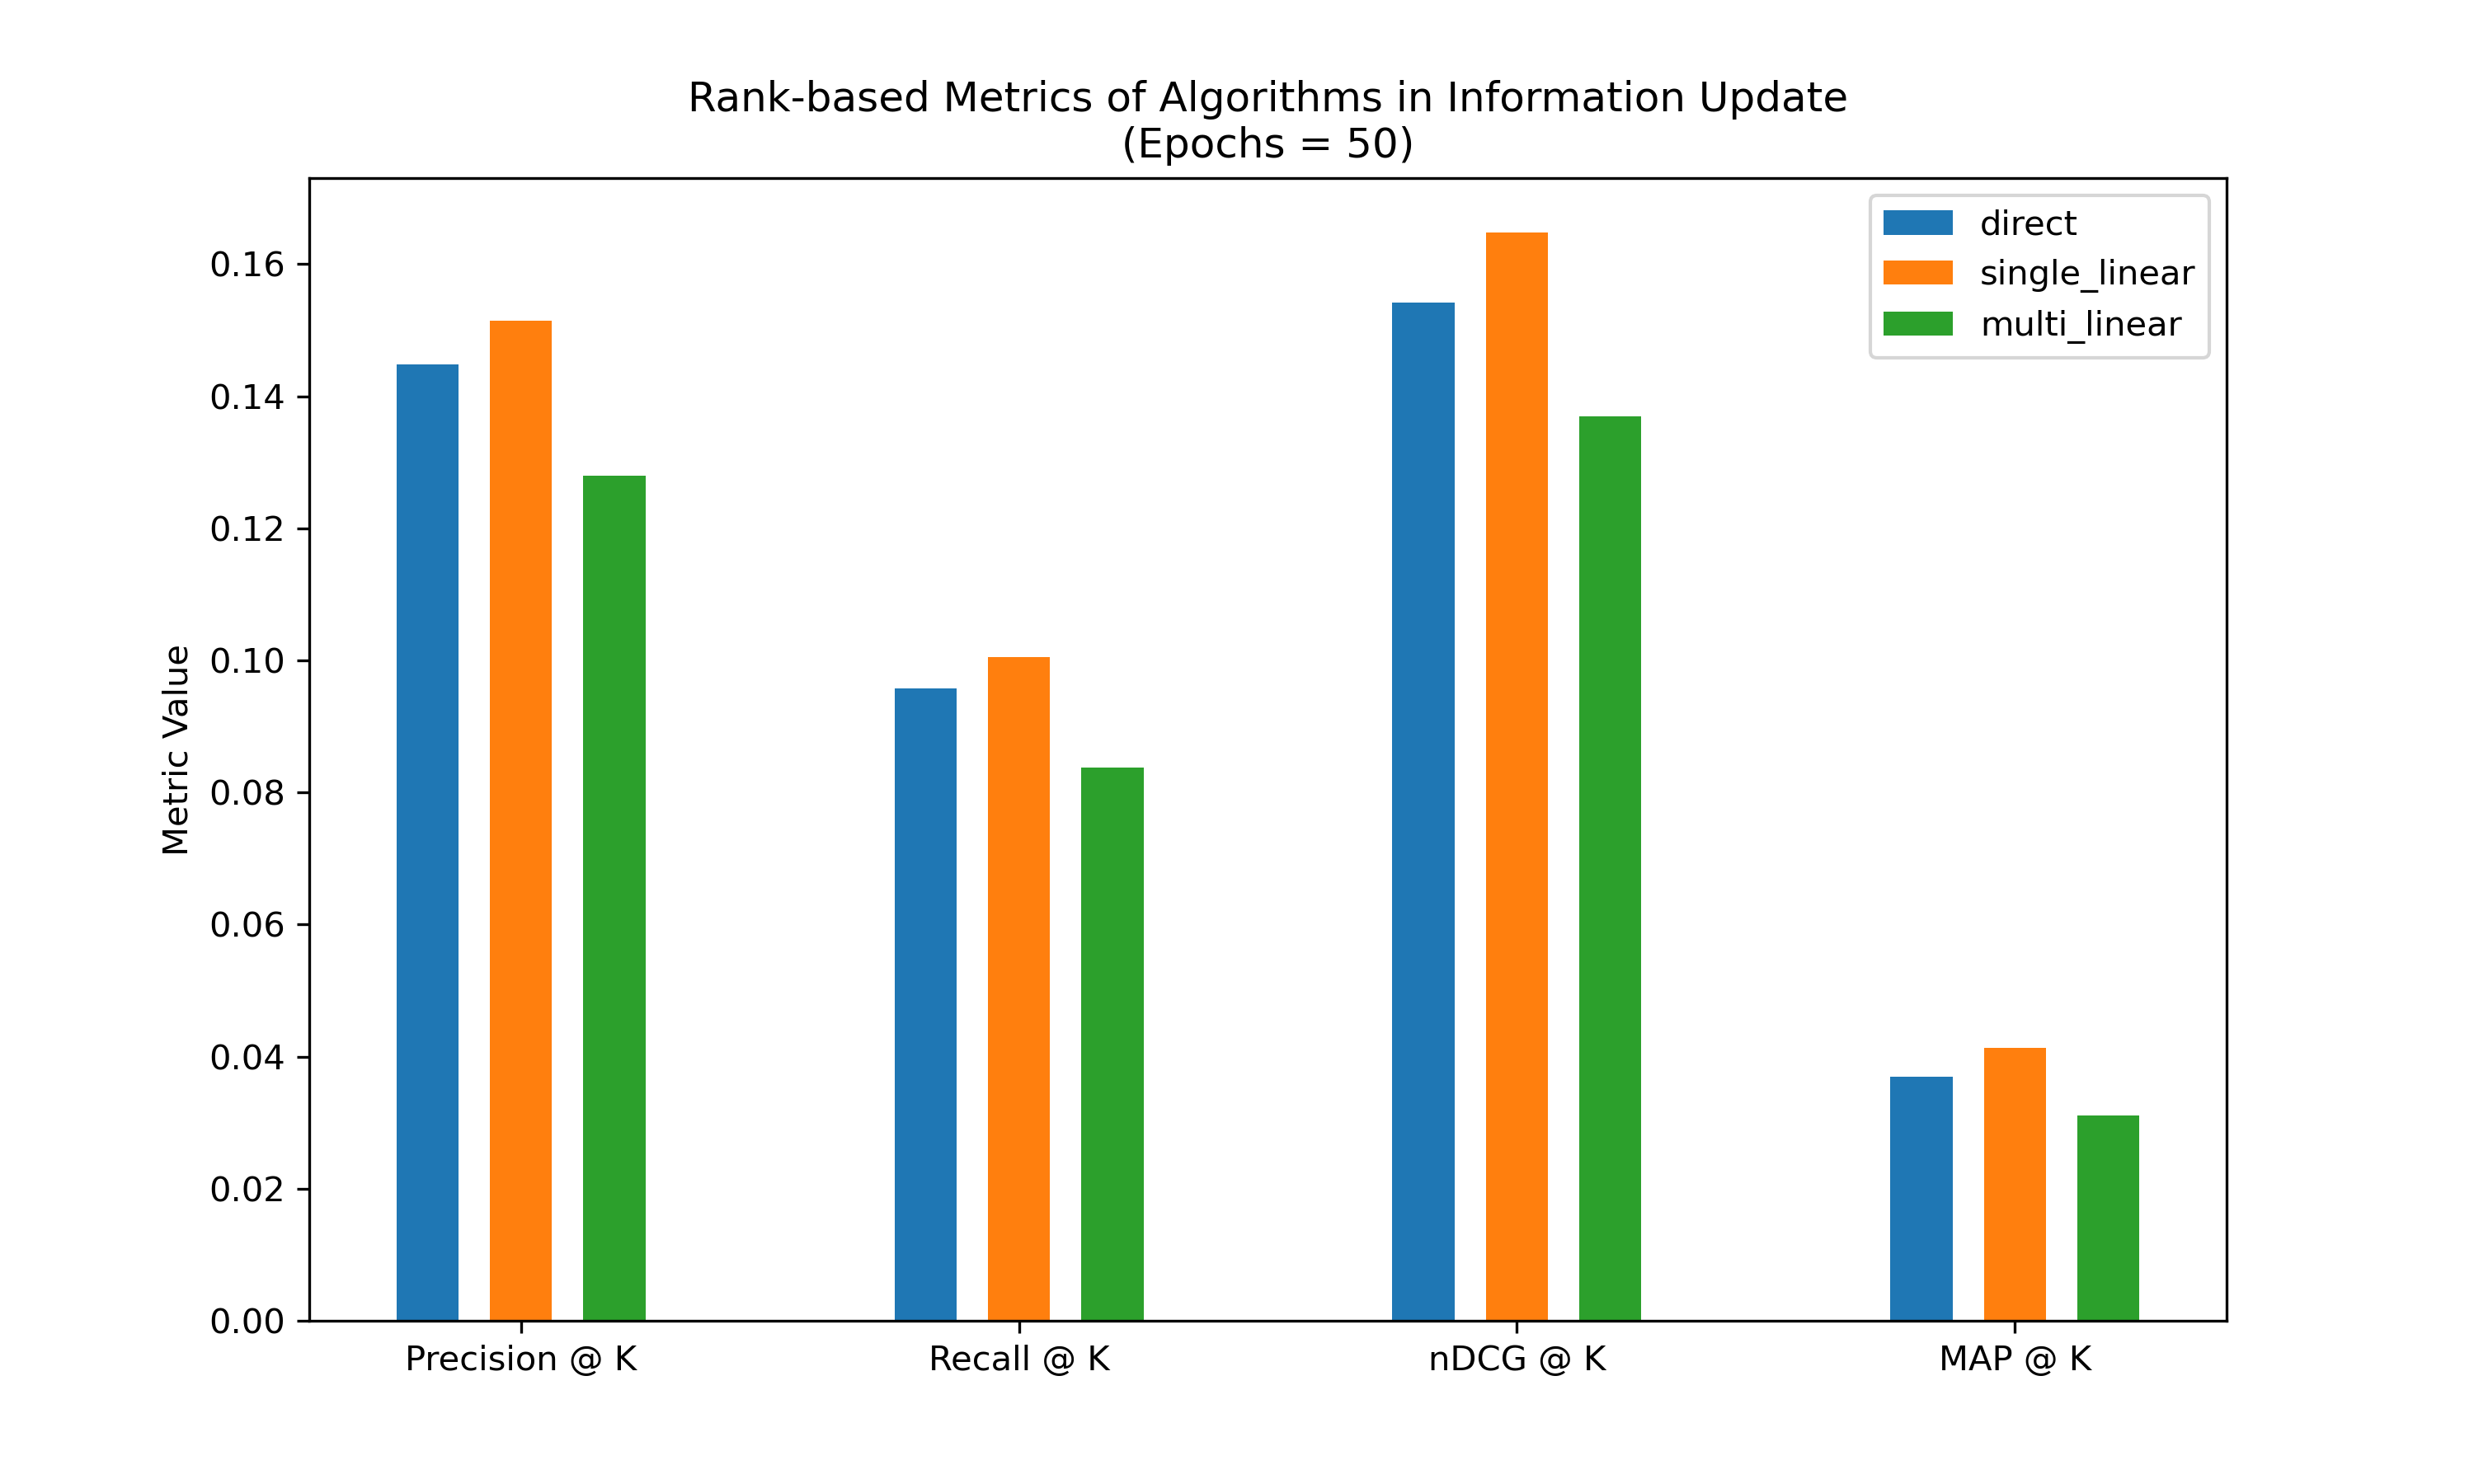
\includegraphics[width=.48\textwidth]{figs/info_updater.png}
    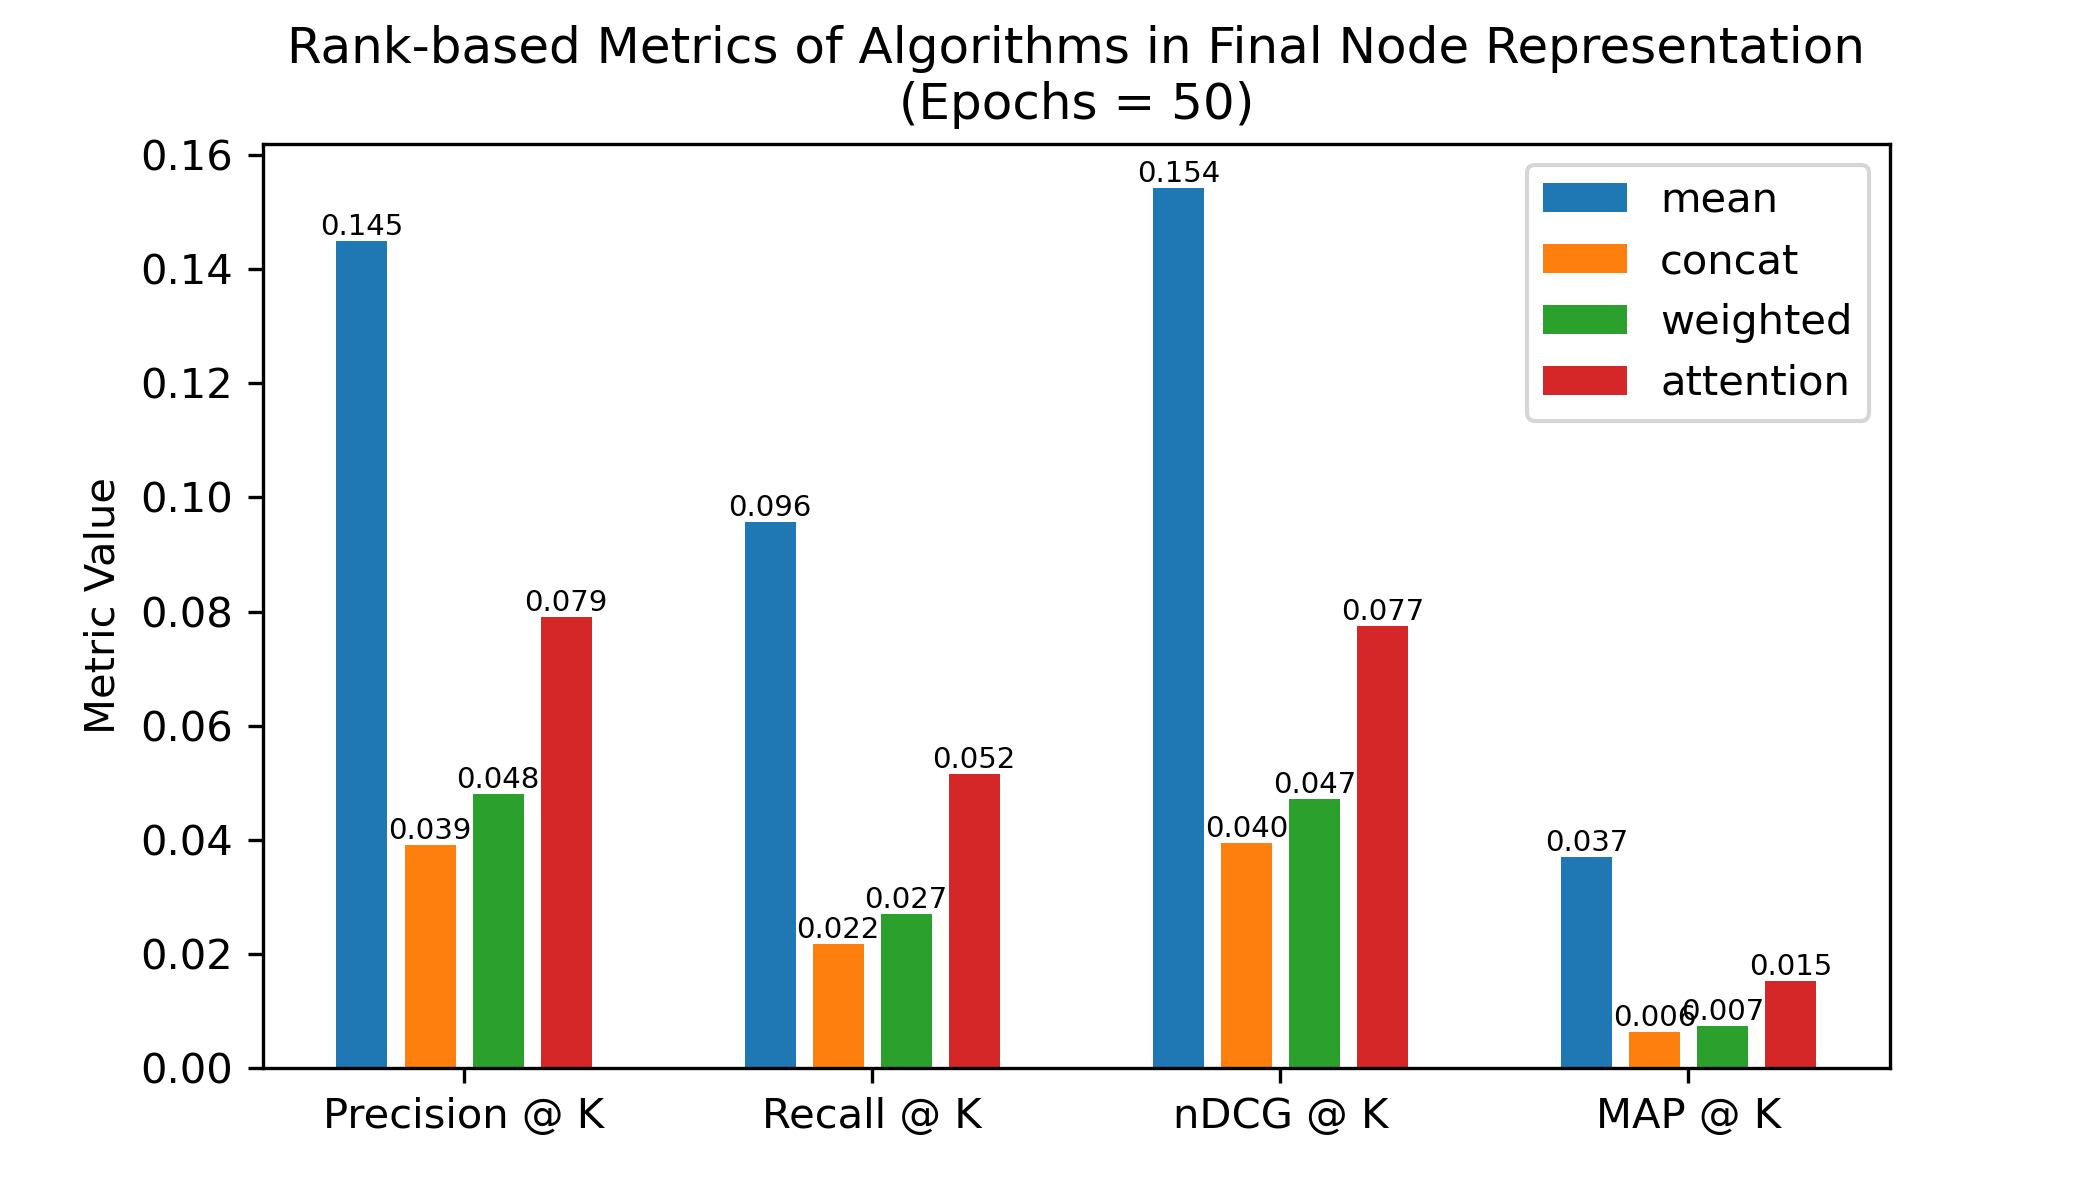
\includegraphics[width=.48\textwidth]{figs/final_node_repr.png}
    \caption{}
    \label{fig:metrics-individual-mechanisms}
\end{figure}

% \begin{figure}[H]
%     % \centering
%     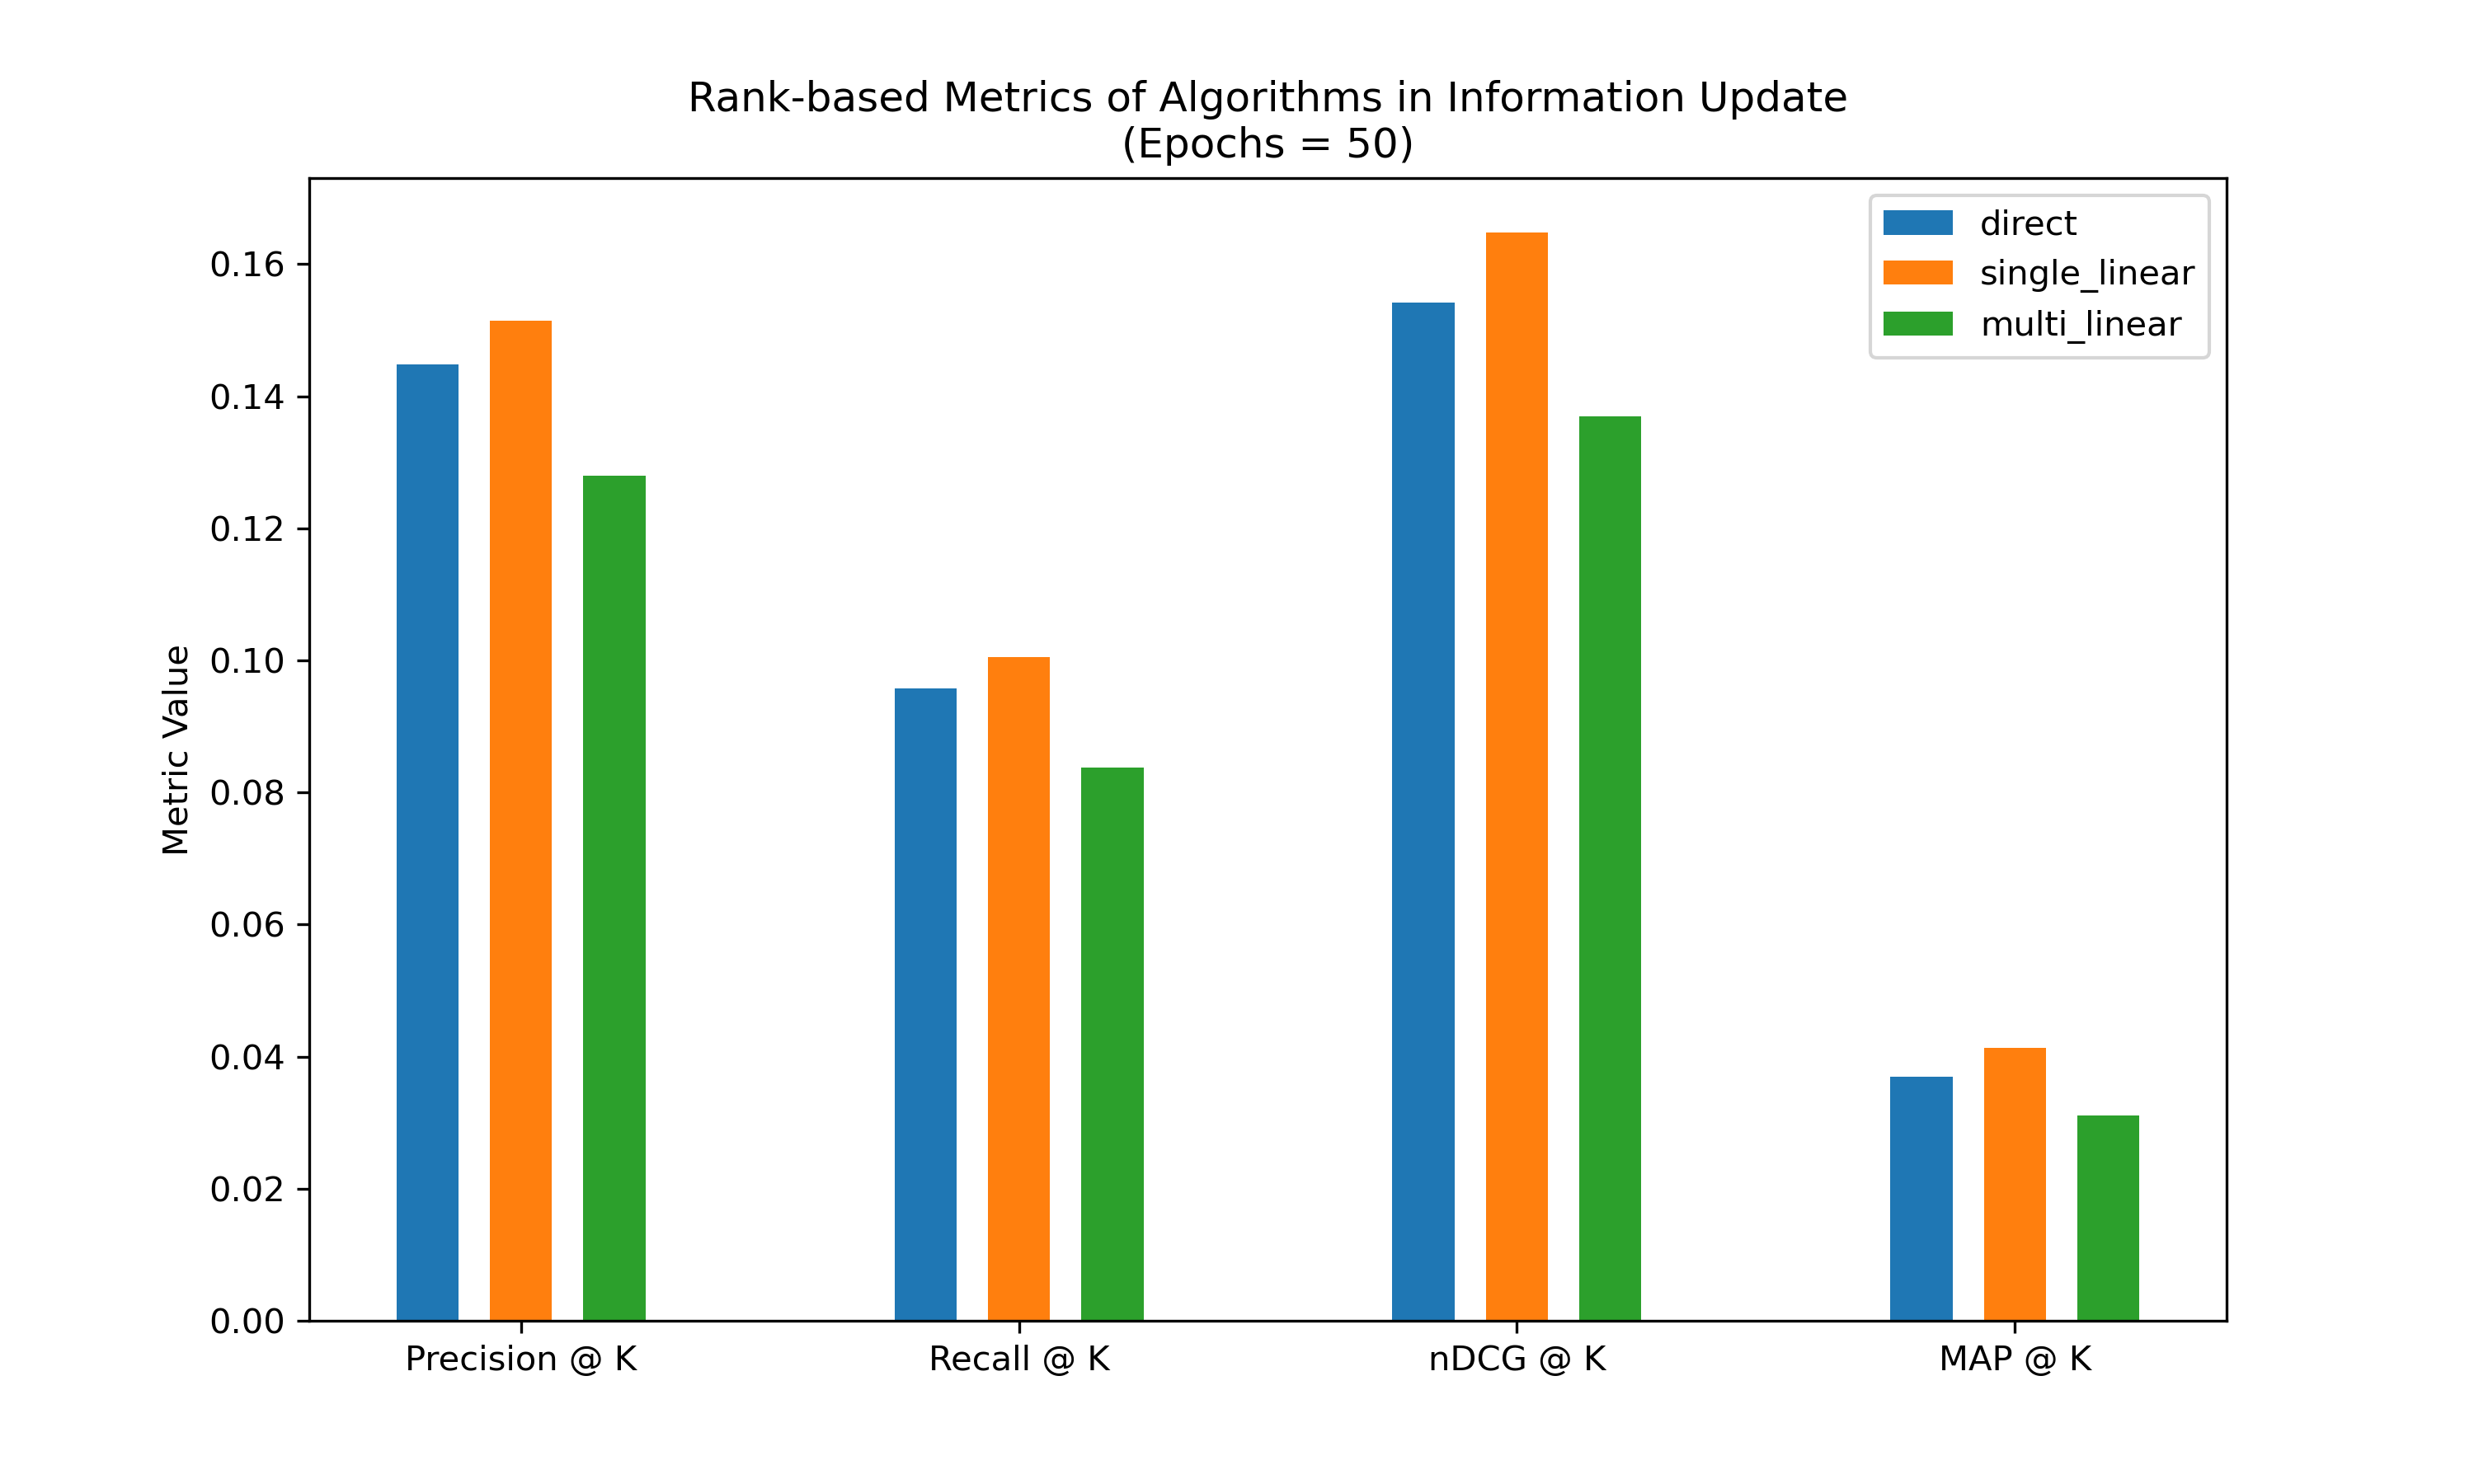
\includegraphics[width=.3\textwidth]{figs/info_updater.png}
%     % \caption{}
%     \label{fig:metrics-info-updater}
% \end{figure}

% \begin{figure}[H]
%     % \centering
%     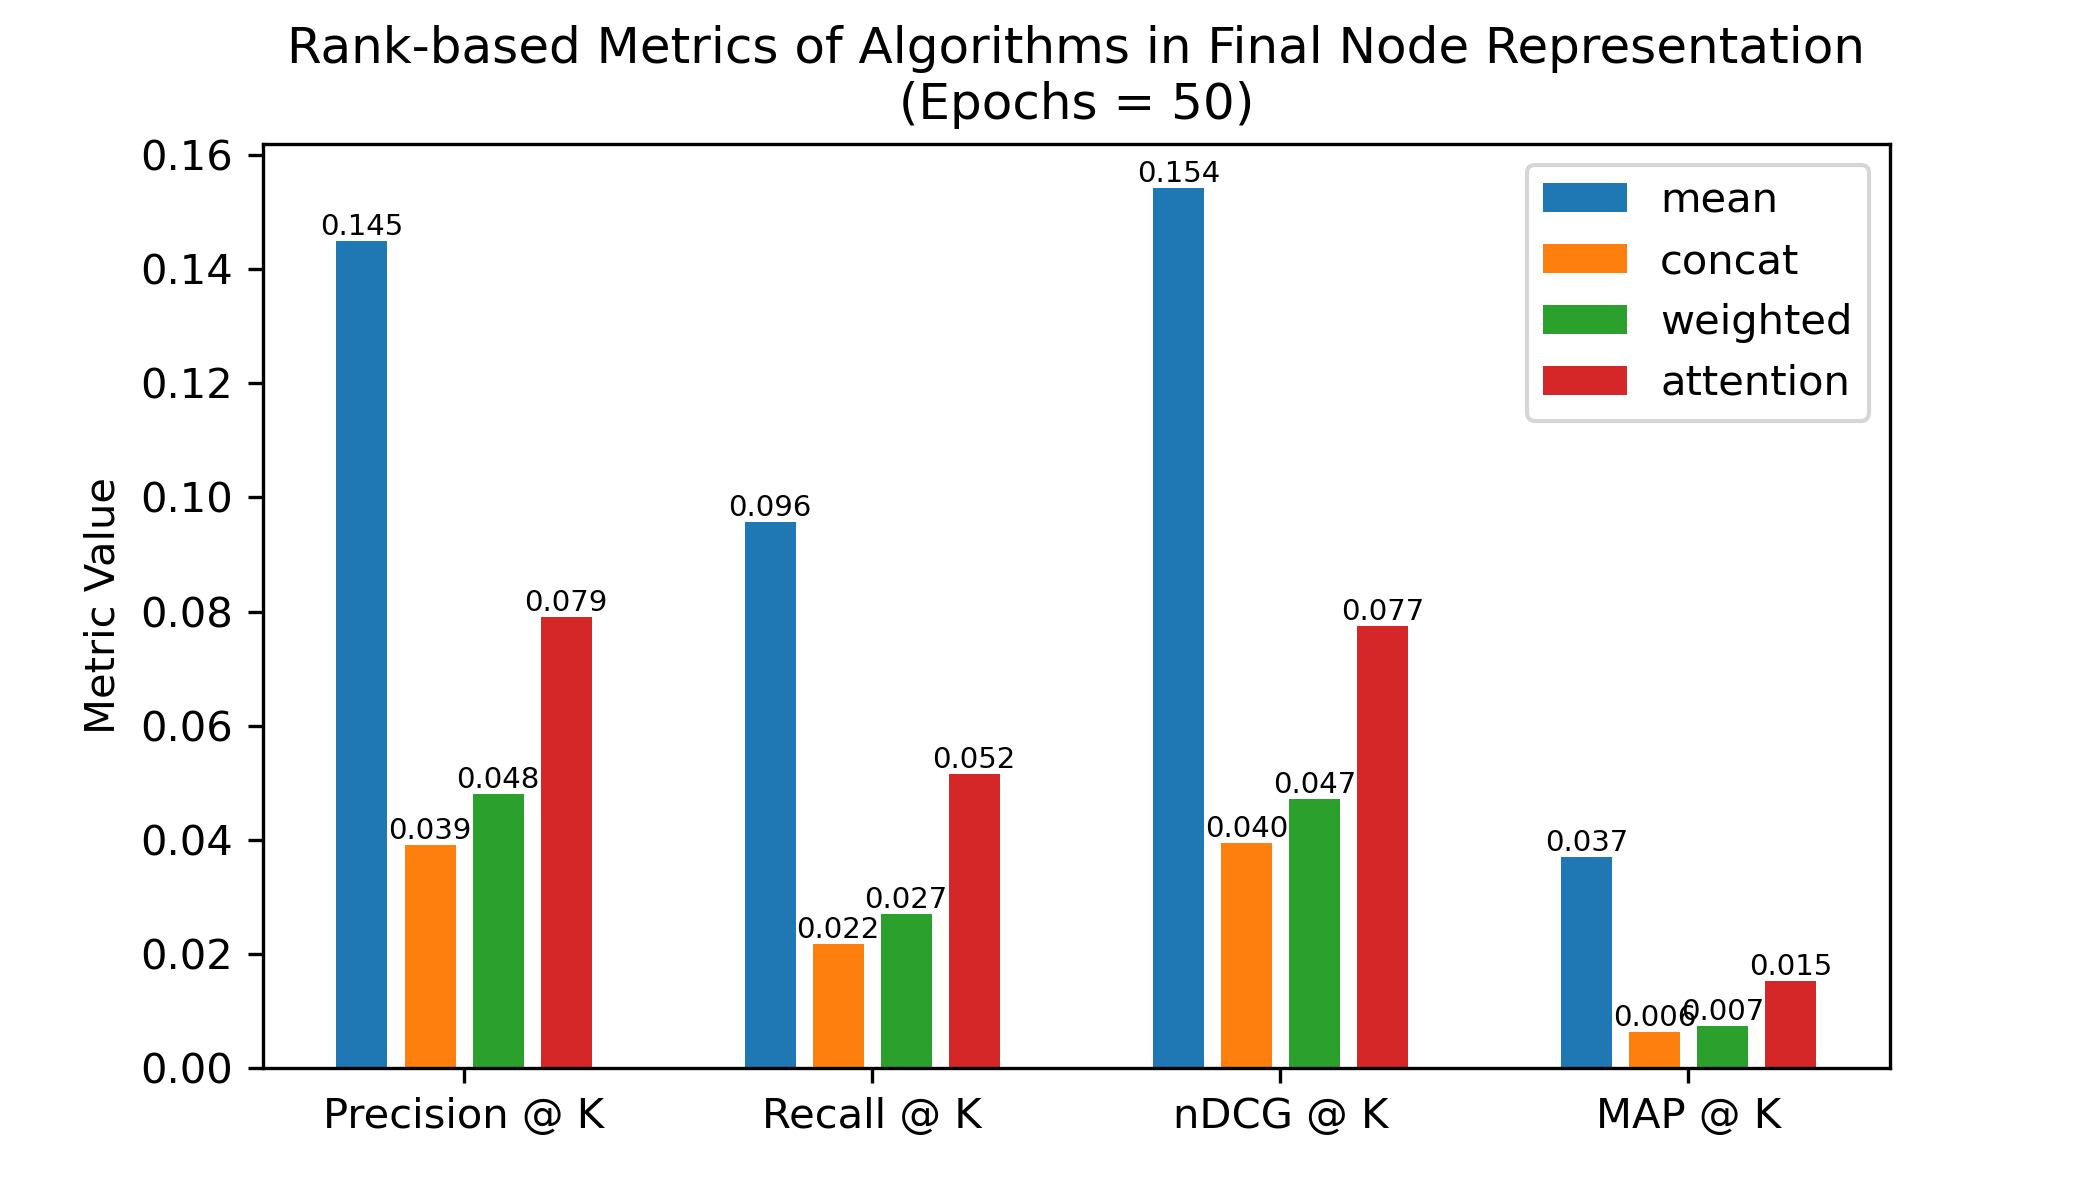
\includegraphics[width=.3\textwidth]{figs/final_node_repr.png}
%     \caption{}
%     \label{fig:metrics-final-node-repr}
% \end{figure}

\subsubsection{Average Normalized Ranking}

% Please add the following required packages to your document preamble:
% \usepackage{multirow}
\begin{table}[H]
\centering
\begin{tabular}{|l|llll|}
\hline
Ranked by                       &                                                                                                           &                                             & Mean           & Stddev \\ \hline
\multirow{9}{*}{NDCG @ 10}      & \multicolumn{1}{l|}{\multirow{2}{*}{\begin{tabular}[c]{@{}l@{}}Neighbor\\ Aggregator\end{tabular}}}       & \multicolumn{1}{l|}{\textbf{attention}}     & \textbf{0.413} & 0.313  \\ \cline{3-5} 
                                & \multicolumn{1}{l|}{}                                                                                     & \multicolumn{1}{l|}{degree norm}            & 0.545          & 0.244  \\ \cline{2-5} 
                                & \multicolumn{1}{l|}{\multirow{3}{*}{\begin{tabular}[c]{@{}l@{}}Information\\ Updater\end{tabular}}}       & \multicolumn{1}{l|}{\textbf{single linear}} & \textbf{0.396} & 0.218  \\ \cline{3-5} 
                                & \multicolumn{1}{l|}{}                                                                                     & \multicolumn{1}{l|}{multi linear}           & 0.500          & 0.222  \\ \cline{3-5} 
                                & \multicolumn{1}{l|}{}                                                                                     & \multicolumn{1}{l|}{identity}               & 0.542          & 0.376  \\ \cline{2-5} 
                                & \multicolumn{1}{l|}{\multirow{4}{*}{\begin{tabular}[c]{@{}l@{}}Final Node\\ Representation\end{tabular}}} & \multicolumn{1}{l|}{\textbf{attention}}     & \textbf{0.271} & 0.277  \\ \cline{3-5} 
                                & \multicolumn{1}{l|}{}                                                                                     & \multicolumn{1}{l|}{mean}                   & 0.312          & 0.175  \\ \cline{3-5} 
                                & \multicolumn{1}{l|}{}                                                                                     & \multicolumn{1}{l|}{weighted}               & 0.535          & 0.195  \\ \cline{3-5} 
                                & \multicolumn{1}{l|}{}                                                                                     & \multicolumn{1}{l|}{concat}                 & 0.799          & 0.106  \\ \hline
\end{tabular}
\caption{}
\label{tab:mechanisms-avg-ranking-ndcg}
\end{table}

Table \ref{tab:mechanisms-avg-ranking}

\textit{compares across all mechanism combinations}

% \subsection{LightGCN: Model Performance Evaluation} \label{lightgcn-eval}

% To evaluate the performance of LightGCN and benchmark it against the baselines, we employ the following rank-based metrics
% $$
% \begin{cases}
% \text{Mean Average Precision (MAP) @ K} \\
% \text{Normalized Discounted Cumulative Gain (nDCG) @ K} \\
% \text{Precision @ K} \\
% \text{Recall @ K}
% \end{cases}
% $$
% For a detailed definition of these metrics, we direct the reader to \cite{metrics}.

% Table \ref{tab:lightgcn-100k-results} summarizes the rank-based metrics for LightGCN as well as the baseline models, which were all trained on the \texttt{MovieLens 100K} dataset. In addition, These results are visualized in Figure \ref{fig:lightgcn-100k-eval}.

% As shown in Figure \ref{fig:lightgcn-100k-eval}, our LightGCN model significantly outperformed all baseline models without even using any complicated non-linear feature transformation. For example, the MAP @ K and Recall @ K of LightGCN are almost two times better than the baselines.

% We believe the main factor that contributed to the success of LightGCN is that it systematically learns the multi-hop relationships in the user-movie interaction graph, which is not utilized by the baseline methods.

%  TO DO: Highlight a few limitations of LightGCN, which could be a nice segway into our next GNN that potentially improves upon LightGCN.

% \textbf{Precision @ K}

% The ``Precision @ K" metric for a recommender model is defined as the proportion of the top K ranks that were correctly predicted. Mathematically, let $R_{u}$ denote the true ranking of user $u$ for her top $K$ favorite movies, and let $\hat{R}_u$ denote the corresponding top-K ranking predicted by the recommender model. Then, its ``Precision @ K" score is
% \begin{align*}
%     \text{Precision @ K} = \frac{1}{M} \sum_{u = 1}^M \frac{1}{K} \sum_{r = 1}^k \delta(R_u[r] = \hat{R}_u[r])
% \end{align*}
% where $\delta(\cdot)$ is the indicator function.

% \textbf{Mean Average Precision @ K}

% The ``Mean Average Precision @ K" metric is simply the average of ``Precision @ k" over $k = 1, 2, \hdots, K$. Mathematically, MAP @ K is defined as
% \begin{align*}
%     \text{MAP @ K} = \frac{1}{K} \sum_{k = 1}^K \text{Prediction @ $k$}
% \end{align*}

\section{Discussion and Analysis}

\textit{Analyze your model and results. Highlight a few limitations of your approach (e.g., strong assumptions you had to make, constraints, when your method did not work in practice, etc.). Do
the results and the explanation provide insights into the ML models or the environment that you were dealing with? Comment on whether you think there is a way to further improve your method to eliminate these limitations.}

\subsection{GNN Paradigm: Analysis of the Individual Components}

\subsubsection{Neighbor Aggregation Algorithms (Tianyu)}

\subsubsection{Information Update Algorithms (Albert)}



\subsubsection{Final Node Representation Algorithms (Hiroshi)}

\subsubsection{A Note on Graph Construction (Hiroshi)}

\textit{a brief discussion on why it didn't work should suffice since we didnt systematically evaluate this}

\subsection{Overall Best-Performing Architectures}


\subsection{Limitations and Future Work}

% Table \ref{tab:rmse_results}, \ref{tab:mae_results} show the 5-fold cross-validation RMSE and MAE of the baseline algorithms, respectively. Figure \ref{fig:rmse-baselines}, \ref{fig:mae-baselines} plots the mean RMSE and MAE against the baseline algorithms, respectively.

% % \section{Evaluation of Preliminary Work}

% From Figure \ref{fig:rmse-baselines} and \ref{fig:mae-baselines}, we see that all four non-trivial baselines beat Random Guess by a large margin. Among them, SVD performs the best in both RMSE and MAE, followed by SlopeOne, NMF, and then k-NN. We note that the different methods do provide non-trivial improvements to the metrics, suggesting there is still room for improvement by employing more sophisticated algorithms, such as GNN.

% \section{Next Steps}

% For our next steps, we would like to further review the literature of neural network in recommendation systems, especially the use of graph neural networks, and start implementing many of them. Starting from basic GNNs such as GraphSAGE \cite{graphsage}, GGNN \cite{ggnn} and GAT \cite{gat}, we plan to experiment with different aspects of the networks such as neighborhood depth, graph structure, etc. We will devise architectures that train GNN together with traditional networks in an end-to-end manner and run ablation experiments to study the additional benefits GNN brings to solving the task. We hope to run these on the same dataset with the same benchmarking and produce better results than the baseline. We will also try these on a bigger dataset like MovieLens1M or MovieLens20M to see if this affects the accuracy of the baseline vs GNN results.

\section{Teammates and Work Division}

% For the rest of the work, we each will first implement a GNN, e.g. GraphSAGE for Albert, GGNN for Hiroshi, and GAT for Tianyu, and evaluate their performance in similar methods as above. This will be done by Nov 11. Then, we individually will explore ways to integrate GNN into traditional neural nets to create more complex architectures that potentially perform better and offers opportunities for more sophisticated analyses (e.g. an ablation study by toggling the GNN module in the whole net on and off). This will be done by Dec 2. We will work on the final draft in the last week leading to Dec 8, the submission deadline.

Every member of the team contributed heavily to this project. We split the implementation of network architectural mechanisms with Tianyu on neighbor aggregation, Albert on information update, and Hiroshi on final node representation and graph construction. Apart from the core code, Albert was heavily involved with the initial setup of the training and evaluation pipeline and results plotting functionalities, Tianyu with experiment infrastructure and metrics analysis, and Hiroshi with auto experimentation functionalities and metrics processing. We co-authored this project's final report.

\section{Access to Code}

% \textit{If relevant to your project, you must provide a link to a Github repository which contains all code used in your project. The repository should contain a README file which explains how to run your code and it should provide a link to your dataset used so that TAs can replicate your work.}

The code to train, plot, and analyze the models is published at the \href{https://github.com/thisisalbertliang/gnn-rec}{GNN-Rec} GitHub repo.

\newpage

\section{Appendix}

\subsection{Rank-based Metrics Definitions} \label{rank-metrics-def}

\subsubsection{Precision @ K}

For a given user $u$, Precision @ K measures the fraction of the top K items recommended by the model that are relevant to the user. Mathematically, it is defined as \cite{survey}:
$$
\mbox{Precision@K}(u) = \frac{| R^K(u) \cap T(u) |}{K}
$$
where $R^K(u)$ is the set of top K items ranked by the model for user $u$, and $T(u)$ is the ground truth set of top K items for user $u$. If we do not specify the user $u$, then we are referring to the average Precision @ K across all users, i.e. $\mbox{Precision@K} = \frac{1}{M} \sum_{u = 1}^M \mbox{Precision@K(u)}$.

\subsubsection{Recall @ K}

Recall @ K measures the fraction of the top K items recommended by the model that are in the ground truth set of top K items for the user. Mathematically, it is defined as \cite{survey}:
$$
\mbox{Recall@K}(u) = \frac{| R^K(u) \cap T(u) |}{|T(u)|}
$$
Similarly, if we do not specify the user $u$, then we are referring to the average Recall @ K across all users, i.e. $\mbox{Recall@K} = \frac{1}{M} \sum_{u = 1}^M \mbox{Recall@K(u)}$.

\subsubsection{Normalized Discounted Cumulative Gain (nDCG) @ K}

Normalized Discounted Cumulative Gain (nDCG) @ K measures the ranking quality of the top K recommended items by differentiating the contributions of correctly recommended items based on their ranking positions. Mathematically, it is defined as \cite{survey}:
$$
\mbox{nDCG@K} = \frac{1}{M} \sum_{u = 1}^M \frac{\sum_{k = 1}^K \frac{I(R^K_k(u) \in T(u))}{\log(k + 1)}}{\sum_{k = 1}^K \frac{1}{ \log(k + 1)}}
$$
where $I(\cdot)$ is the indicator function, $R^K_k(u)$ is the $k$th item in the top K items ranked by the model for user $u$, and $T(u)$ is the ground truth set of top K items for user $u$. The denominator is the ideal DCG score if the top K items are perfectly ranked by the model.

\subsubsection{Mean Average Precision (MAP) @ K}

Mean Average Precision (MAP) @ K is the average of the Precision @ K across all users for multiple queries. Mathematically, it is defined as \cite{survey}:
$$
\mbox{MAP@K} = \frac{1}{M} \sum_{u = 1}^M \sum_{k = 1}^K \frac{I(R^K_k(u) \in T(u)) \mbox{Precision@K}(u)}{K}
$$


\subsection{Additional Baseline Evaluations} \label{additional-baseline-eval}

\begin{table}[H]
    \centering
        \begin{tabular}{|c c c c c c c|} 
         \hline
         Baseline & Fold 1 & Fold 2 & Fold 3 & Fold 4 & Fold 5 & Mean \\ [0.5ex] 
         \hline\hline
         SVD & 0.935 & 0.928 & 0.931 & 0.932 & 0.946 & \bfseries 0.934 \\ 
         \hline
         NMF & 0.964 & 0.962 & 0.957 & 0.961 & 0.973 & 0.963 \\
         \hline
         SlopeOne & 0.947 & 0.941 & 0.941 & 0.942 & 0.958 & 0.946 \\
         \hline
         k-NN & 0.984 & 0.975 & 0.976 & 0.975 & 0.987 & 0.980 \\
         \hline
         Random Guess & 1.514 & 1.519 & 1.524 & 1.509 & 1.524 & 1.518 \\ [1ex] 
         \hline
        \end{tabular}
    \caption{5 Fold Cross Validation RMSE of Baseline Algorithms}
    \label{tab:rmse_results}
\end{table}

\begin{table}[H]
    \centering
        \begin{tabular}{|c c c c c c c|} 
         \hline
         Baseline & Fold 1 & Fold 2 & Fold 3 & Fold 4 & Fold 5 & Mean \\ [0.5ex] 
         \hline\hline
         SVD & 0.737 & 0.731 & 0.735 & 0.734 & 0.747 & \bfseries 0.737 \\ 
         \hline
         NMF & 0.759 & 0.758 & 0.754 & 0.754 & 0.765 & 0.758 \\
         \hline
         SlopeOne & 0.744 & 0.740 & 0.740 & 0.740 & 0.753 & 0.743 \\
         \hline
         k-NN & 0.776 & 0.771 & 0.770 & 0.769 & 0.782 & 0.774 \\
         \hline
         Random Guess & 1.215 & 1.221 & 1.225 & 1.210 & 1.223 & 1.219 \\ [1ex] 
         \hline
        \end{tabular}
    \caption{5 Fold Cross Validation MAE of Baseline Algorithms}
    \label{tab:mae_results}
\end{table}

% \begin{table}[H]
%     \centering
%         \begin{tabular}{|c c c c c c c|} 
%          \hline
%          Baseline & Fold 1 & Fold 2 & Fold 3 & Fold 4 & Fold 5 & Mean \\ [0.5ex] 
%          \hline\hline
%          SVD & 0.737 & 0.731 & 0.735 & 0.734 & 0.747 & \bfseries 0.737 \\ 
%          \hline
%          NMF & 0.759 & 0.758 & 0.754 & 0.754 & 0.765 & 0.758 \\
%          \hline
%          SlopeOne & 0.744 & 0.740 & 0.740 & 0.740 & 0.753 & 0.743 \\
%          \hline
%          k-NN & 0.776 & 0.771 & 0.770 & 0.769 & 0.782 & 0.774 \\
%          \hline
%          Random Guess & 1.215 & 1.221 & 1.225 & 1.210 & 1.223 & 1.219 \\ [1ex] 
%          \hline
%         \end{tabular}
%     \caption{5 Fold Cross Validation MAE of Baseline Algorithms}
%     \label{tab:mae_results}
% \end{table}

% \begin{figure}[H]
%     \centering
%     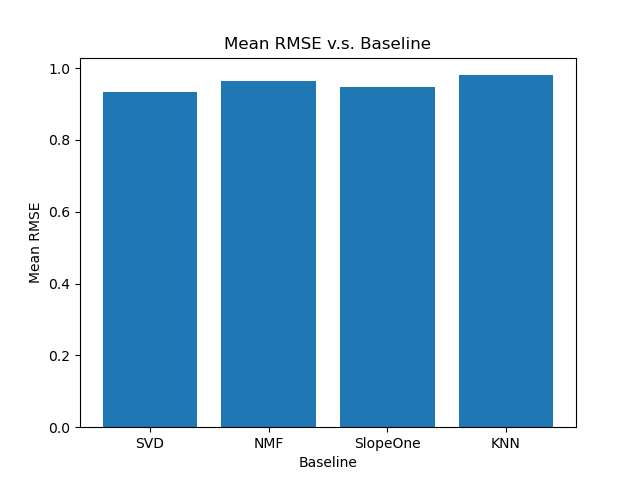
\includegraphics[width=.8\textwidth]{figs/rmse-baselines.png}
%     \caption{5 Fold Cross Validation: Mean RMSE v.s. Baselines}
%     \label{fig:rmse-baselines}
% \end{figure}

% \begin{figure}[H]
%     \centering
%     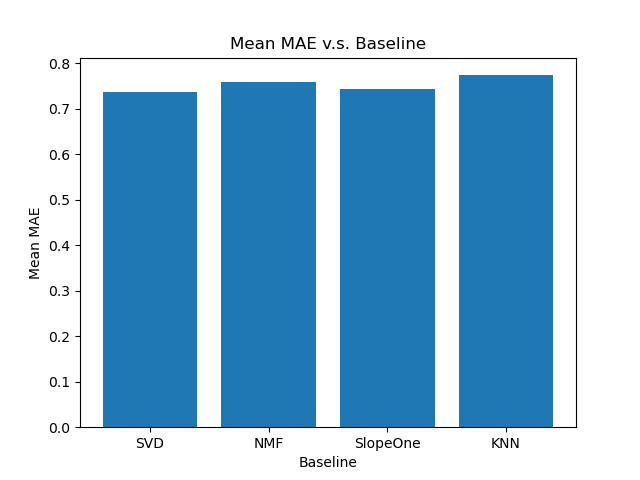
\includegraphics[width=.8\textwidth]{figs/mae-baselines.png}
%     \caption{5 Fold Cross Validation: Mean MAE v.s. Baselines}
%     \label{fig:mae-baselines}
% \end{figure}

% \begin{figure}
%     \centering
%     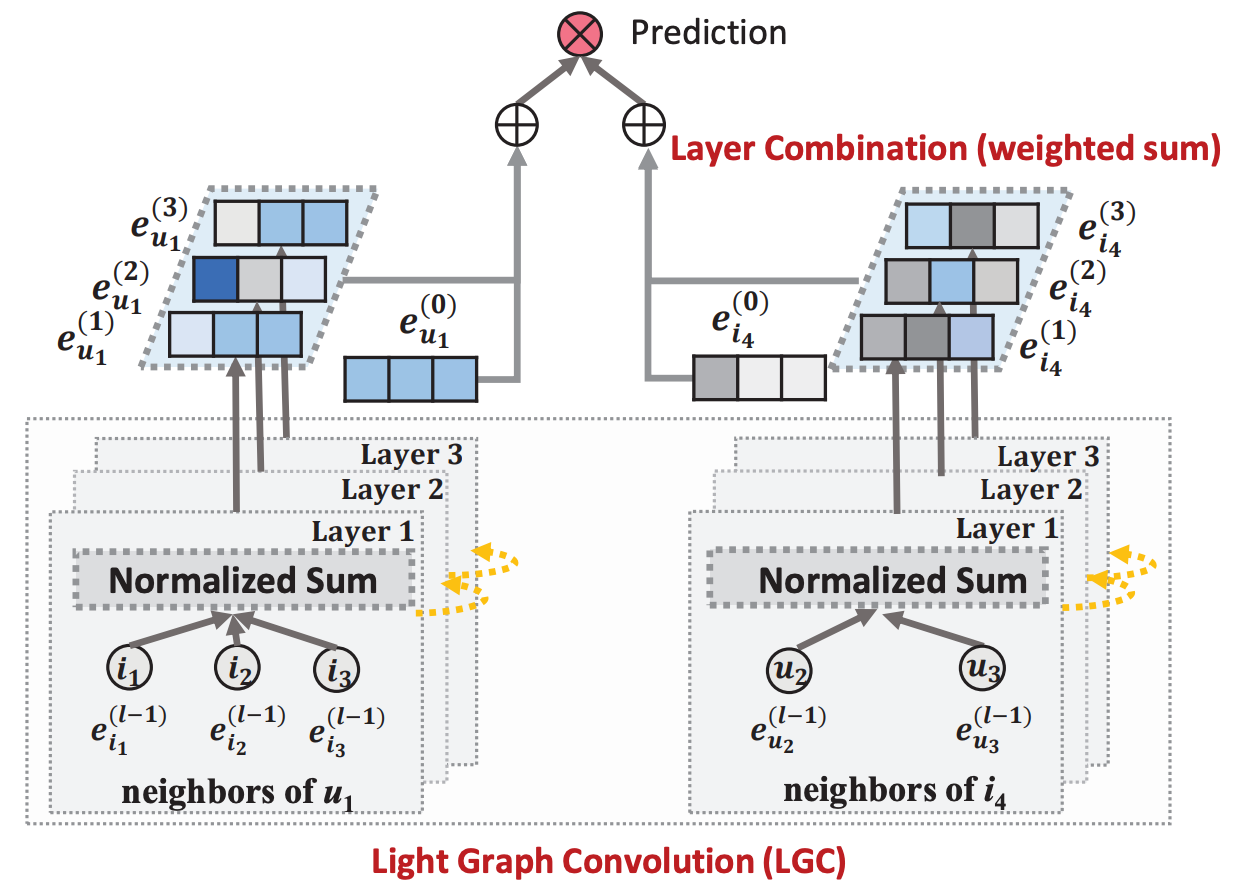
\includegraphics[width=.8\textwidth]{figs/light-gcn-architecture.png}
%     \caption{An illustration of the LightGCN architecture from \cite{lightgcn}. In LightGCN, the current layer only passes the normalized sum of the neighbor embeddings to the next layer. LightGCN throws away all other operations such as self-connection, feature transformation, and non-linear activation that are commonly seen in GCN. At the layer combination stage, LightGCN computes the final embedding as the weighted average of the embeddings at each layer}
%     \label{fig:light-gcn-architecture}
% \end{figure}



% \begin{figure}[H]
%     \centering
%     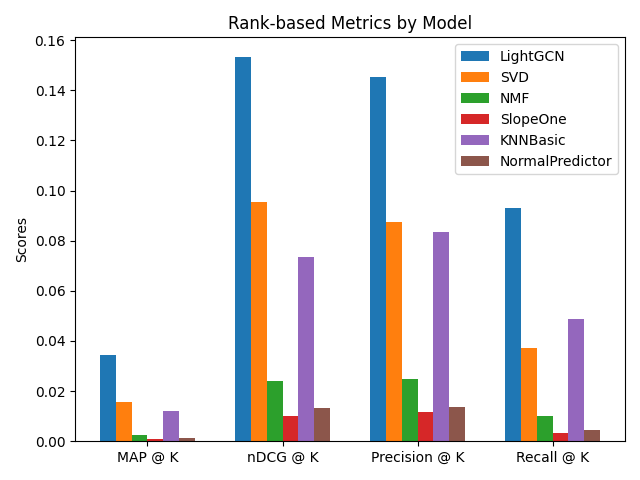
\includegraphics[width=.8\textwidth]{figs/lightgcn-movielens100k-eval.png}
%     \caption{A visualization of the results from Table \ref{tab:lightgcn-100k-results}.}
%     \label{fig:lightgcn-100k-eval}
% \end{figure}


\subsection{Additional GNN Evaluation Tables and Plots} \label{additional-gnn-eval}

% Please add the following required packages to your document preamble:
% \usepackage{multirow}
\begin{table}[H]
\centering
\begin{tabular}{|l|llll|}
\hline
Ranked by                       &                                                                                                           &                                             & Mean           & Stddev \\ \hline
\multirow{9}{*}{Recall @ 10}    & \multicolumn{1}{l|}{\multirow{2}{*}{\begin{tabular}[c]{@{}l@{}}Neighbor\\ Aggregator\end{tabular}}}       & \multicolumn{1}{l|}{\textbf{attention}}     & \textbf{0.431} & 0.294  \\ \cline{3-5} 
                                & \multicolumn{1}{l|}{}                                                                                     & \multicolumn{1}{l|}{degree norm}            & 0.528          & 0.274  \\ \cline{2-5} 
                                & \multicolumn{1}{l|}{\multirow{3}{*}{\begin{tabular}[c]{@{}l@{}}Information\\ Updater\end{tabular}}}       & \multicolumn{1}{l|}{\textbf{single linear}} & \textbf{0.391} & 0.221  \\ \cline{3-5} 
                                & \multicolumn{1}{l|}{}                                                                                     & \multicolumn{1}{l|}{multi linear}           & 0.505          & 0.216  \\ \cline{3-5} 
                                & \multicolumn{1}{l|}{}                                                                                     & \multicolumn{1}{l|}{identity}               & 0.542          & 0.376  \\ \cline{2-5} 
                                & \multicolumn{1}{l|}{\multirow{4}{*}{\begin{tabular}[c]{@{}l@{}}Final Node\\ Representation\end{tabular}}} & \multicolumn{1}{l|}{\textbf{attention}}     & \textbf{0.299} & 0.263  \\ \cline{3-5} 
                                & \multicolumn{1}{l|}{}                                                                                     & \multicolumn{1}{l|}{mean}                   & 0.306          & 0.186  \\ \cline{3-5} 
                                & \multicolumn{1}{l|}{}                                                                                     & \multicolumn{1}{l|}{weighted}               & 0.514          & 0.228  \\ \cline{3-5} 
                                & \multicolumn{1}{l|}{}                                                                                     & \multicolumn{1}{l|}{concat}                 & 0.799          & 0.106  \\ \hline
\multirow{9}{*}{nDCG @ 10}      & \multicolumn{1}{l|}{\multirow{2}{*}{\begin{tabular}[c]{@{}l@{}}Neighbor\\ Aggregator\end{tabular}}}       & \multicolumn{1}{l|}{\textbf{attention}}     & \textbf{0.413} & 0.313  \\ \cline{3-5} 
                                & \multicolumn{1}{l|}{}                                                                                     & \multicolumn{1}{l|}{degree norm}            & 0.545          & 0.244  \\ \cline{2-5} 
                                & \multicolumn{1}{l|}{\multirow{3}{*}{\begin{tabular}[c]{@{}l@{}}Information\\ Updater\end{tabular}}}       & \multicolumn{1}{l|}{\textbf{single linear}} & \textbf{0.396} & 0.218  \\ \cline{3-5} 
                                & \multicolumn{1}{l|}{}                                                                                     & \multicolumn{1}{l|}{multi linear}           & 0.500          & 0.222  \\ \cline{3-5} 
                                & \multicolumn{1}{l|}{}                                                                                     & \multicolumn{1}{l|}{identity}               & 0.542          & 0.376  \\ \cline{2-5} 
                                & \multicolumn{1}{l|}{\multirow{4}{*}{\begin{tabular}[c]{@{}l@{}}Final Node\\ Representation\end{tabular}}} & \multicolumn{1}{l|}{\textbf{attention}}     & \textbf{0.271} & 0.277  \\ \cline{3-5} 
                                & \multicolumn{1}{l|}{}                                                                                     & \multicolumn{1}{l|}{mean}                   & 0.312          & 0.175  \\ \cline{3-5} 
                                & \multicolumn{1}{l|}{}                                                                                     & \multicolumn{1}{l|}{weighted}               & 0.535          & 0.195  \\ \cline{3-5} 
                                & \multicolumn{1}{l|}{}                                                                                     & \multicolumn{1}{l|}{concat}                 & 0.799          & 0.106  \\ \hline
\multirow{9}{*}{Precision @ 10} & \multicolumn{1}{l|}{\multirow{2}{*}{\begin{tabular}[c]{@{}l@{}}Neighbor\\ Aggregator\end{tabular}}}       & \multicolumn{1}{l|}{\textbf{attention}}     & \textbf{0.413} & 0.312  \\ \cline{3-5} 
                                & \multicolumn{1}{l|}{}                                                                                     & \multicolumn{1}{l|}{degree norm}            & 0.545          & 0.246  \\ \cline{2-5} 
                                & \multicolumn{1}{l|}{\multirow{3}{*}{\begin{tabular}[c]{@{}l@{}}Information\\ Updater\end{tabular}}}       & \multicolumn{1}{l|}{\textbf{single linear}} & \textbf{0.401} & 0.223  \\ \cline{3-5} 
                                & \multicolumn{1}{l|}{}                                                                                     & \multicolumn{1}{l|}{multi linear}           & 0.500          & 0.213  \\ \cline{3-5} 
                                & \multicolumn{1}{l|}{}                                                                                     & \multicolumn{1}{l|}{identity}               & 0.536          & 0.380  \\ \cline{2-5} 
                                & \multicolumn{1}{l|}{\multirow{4}{*}{\begin{tabular}[c]{@{}l@{}}Final Node\\ Representation\end{tabular}}} & \multicolumn{1}{l|}{\textbf{attention}}     & \textbf{0.271} & 0.277  \\ \cline{3-5} 
                                & \multicolumn{1}{l|}{}                                                                                     & \multicolumn{1}{l|}{mean}                   & 0.299          & 0.169  \\ \cline{3-5} 
                                & \multicolumn{1}{l|}{}                                                                                     & \multicolumn{1}{l|}{weighted}               & 0.549          & 0.182  \\ \cline{3-5} 
                                & \multicolumn{1}{l|}{}                                                                                     & \multicolumn{1}{l|}{concat}                 & 0.799          & 0.106  \\ \hline
\multirow{9}{*}{MAP @ 10}       & \multicolumn{1}{l|}{\multirow{2}{*}{\begin{tabular}[c]{@{}l@{}}Neighbor\\ Aggregator\end{tabular}}}       & \multicolumn{1}{l|}{\textbf{attention}}     & \textbf{0.417} & 0.311  \\ \cline{3-5} 
                                & \multicolumn{1}{l|}{}                                                                                     & \multicolumn{1}{l|}{degree norm}            & 0.542          & 0.249  \\ \cline{2-5} 
                                & \multicolumn{1}{l|}{\multirow{3}{*}{\begin{tabular}[c]{@{}l@{}}Information\\ Updater\end{tabular}}}       & \multicolumn{1}{l|}{\textbf{single linear}} & \textbf{0.391} & 0.221  \\ \cline{3-5} 
                                & \multicolumn{1}{l|}{}                                                                                     & \multicolumn{1}{l|}{multi linear}           & 0.500          & 0.220  \\ \cline{3-5} 
                                & \multicolumn{1}{l|}{}                                                                                     & \multicolumn{1}{l|}{identity}               & 0.547          & 0.373  \\ \cline{2-5} 
                                & \multicolumn{1}{l|}{\multirow{4}{*}{\begin{tabular}[c]{@{}l@{}}Final Node\\ Representation\end{tabular}}} & \multicolumn{1}{l|}{\textbf{mean}}          & \textbf{0.292} & 0.198  \\ \cline{3-5} 
                                & \multicolumn{1}{l|}{}                                                                                     & \multicolumn{1}{l|}{attention}              & 0.292          & 0.262  \\ \cline{3-5} 
                                & \multicolumn{1}{l|}{}                                                                                     & \multicolumn{1}{l|}{weighted}               & 0.535          & 0.195  \\ \cline{3-5} 
                                & \multicolumn{1}{l|}{}                                                                                     & \multicolumn{1}{l|}{concat}                 & 0.799          & 0.106  \\ \hline
\end{tabular}
\caption{Average normalized ranking of GNN with various architectural choices evaluated under different rank-based metrics. For each architecture choice, e.g., attention as the neighbor aggregator, we fix this choice and vary the other two choices and compute an average ranking of GNNs with attention as the neighbor aggregator. We then normalize this average ranking with all possible combinations of architectural choices.  A lower score means the GNN is ranked more to the front and is thus better. }
\label{tab:mechanisms-avg-ranking}
\end{table}

\pagebreak

\bibliography{references}{}
\bibliographystyle{plain}

\end{document}
